\documentclass[twoside]{Plantilla}
\newcommand{\newemptypage}{\clearpage\newpage\mbox{}\clearpage\newpage}
\begin{document}

% Portada del TFC
\begin{titlepage}
\vspace*{1.5in}
\begin{center}
\vspace*{-1in}
\begin{figure}[htb]
\begin{center}

\includegraphics[width=8cm]{./images/LogoESI.jpg} 
\end{center}
\end{figure}
\end{center}
\begin{center}
Escuela Superior de Informática \\
Universidad de Castilla-La Mancha \\
\vspace*{0.8in}

\begin{Large}
CURSO DE EXPERTO EN DESARROLLO\\
DE VIDEOJUEGOS \\
\end{Large}

\vspace*{0.8in}
\begin{large}
TRABAJO DE FIN DE CURSO \\
\vspace*{0.8in}
\textit{ALLIANCE} \\
SEPTIEMBRE 2018
\end{large}
\end{center}

\end{titlepage}

% Página en blanco para mantener el formato 'libro'
\newemptypage

% Primera página impar del TFC
\vspace*{1.5in}
\begin{center}
\vspace*{-1in}
\begin{figure}[htb]
\begin{center}

\includegraphics[width=8cm]{./images/LogoESI.jpg} 
\end{center}
\end{figure}
\end{center}
\begin{center}
Escuela Superior de Informática \\
Universidad de Castilla-La Mancha \\
\vspace*{0.8in}

\begin{Large}
CURSO DE EXPERTO EN DESARROLLO\\
DE VIDEOJUEGOS \\
\end{Large}

\vspace*{0.8in}
\begin{large}
TRABAJO DE FIN DE CURSO \\
\textit{ALLIANCE} \\

\vspace*{0.6in}
Córdoba Romero, Javier \\
Corroto Martín, Juan José\\
García Herrera, Iván\\

\vspace*{0.4in}
SEPTIEMBRE 2018
\end{large}
\end{center}

\newemptypage

% Segunda página impar del TFC. Anexo III. página de calificación del TFC
\setlength{\parskip}{0mm}

\begin{figure}[htb]

\includegraphics[width=5cm]{./images/LogoESILetras.jpg}
\end{figure}

\begin{center}
CURSO DE EXPERTO EN DESARROLLO DE VIDEOJUEGOS 
\vspace*{0.1in}

\begin{LARGE}Calificación Trabajo Fin de Curso\end{LARGE}
\end{center}

\vspace*{0.2in}

CONVOCATORIA: \hspace*{2.5in} Septiembre 2018 
\vspace*{0.1in}

TÍTULO DEL PROYECTO: \hspace*{1.9in} \textit{ALLIANCE}
\vspace*{0.1in}

AUTORES (ORDEN ALFABÉTICO):
\vspace*{0.1in}

\hspace*{0.5in}Córdoba Romero, Javier \\
\hspace*{0.5in}Corroto Martín, Juan José\\
\hspace*{0.5in}García Herrera, Iván\\

\vspace*{0.2in}
TRIBUNAL:
\vspace*{0.1in}

\hspace*{0.5in}Presidente: \hspace*{0.15in} \rule{100mm}{0.1mm}
\vspace*{0.1in}

\hspace*{0.5in}Vocal: \hspace*{0.47in} \rule{100mm}{0.1mm}
\vspace*{0.1in}


\hspace*{0.5in}Secretario: \hspace*{0.18in} \rule{100mm}{0.1mm}
\vspace*{0.1in}

\vspace*{0.5in}

FECHA DE DEFENSA: \hspace*{0.25in} \rule{87mm}{0.1mm}
\vspace*{0.1in}

CALIFICACIÓN:  \hspace*{0.69in} \rule{87mm}{0.1mm}\\

\vspace*{0.8in}

\hspace*{1in}PRESIDENTE \hspace*{0.6in}VOCAL \hspace*{0.6in}SECRETARIO

\vspace*{1in}

\hspace*{1in}Fdo: \hspace*{1.4in}Fdo: \hspace*{1.3in}Fdo:

\newemptypage

% Índice de Contenidos
\tableofcontents
\newpage

% Índice de Cuadros
\listoftables
\addcontentsline{toc}{section}{\protect\numberline{}Índice de Cuadros}
\newpage

% Índice de Figuras
\listoffigures
\addcontentsline{toc}{section}{\protect\numberline{}Índice de Figuras}
\newpage

% Índice de Listados
\lstlistoflistings
\addcontentsline{toc}{section}{\protect\numberline{}Índice de Listados}
\newpage

% Listado de acrónimos
\section*{Acrónimos}
\addcontentsline{toc}{section}{\protect\numberline{}Acrónimos}

{\small
\begin{acronym}[XXXXXXXX]
  \acro{UE4}	 {Unreal Engine 4}
  \acro{DEV}	 {Asociación de Desarrollo Español de Videojuegos}
  \acro{RV}		 {Realidad Virtual}
  \acro{UDK} 	 {Unreal Development Kit}
  \acro{FPS}	 {First Person Shooter}
  \acro{IA}		 {Inteligencia Artificial}
  \acro{LOD}	 {Level of Detail}
  \acro{LAN}	 {Local Area Network}
  \acro{MMG}	 {Massive Multiplayer Game}
  \acro{SDK}     {Software Development Kit}
  \acro{DLC}	 {Downloadable Content}
  \acro{MMO}	 {Massive Multiplayer Online}
  \acro{CEDV}	 {Curso de Experto en Desarrollo de Videojuegos}
  \acro{GUI}	 {Graphical User Interface}
  \acro{RPC}	 {Remote Procedure Call}
\end{acronym}
}

\newpage

% Sección 1: Resumen del trabajo
\pagestyle{insection}
\section{Resumen del trabajo}
\markboth{Resumen del trabajo}{}
\lettrine[lines=2,findent=2pt,nindent=3pt,loversize=0.1]{\textcolor[gray]{0.4}{E}}{l} trabajo en cuestión se trata de un videojuego de acción en tercera persona, realizado con el motor gráfico \ac{UE4}. El juego ha sido desarrollado usando el lenguaje de programación C++ y extendiendo la funcionalidad del mismo con el lenguaje de \textit{scripting} del motor gráfico, \textit{Blueprints}. El videojuego consiste en una campaña cooperativa con posibilidad de que dos jugadores la completen de forma online. Para ello el videojuego usa el subsistema online de Steam\footnote{https://store.steampowered.com}, por lo que es necesario tener abierto Steam para poder jugar el videojuego. El videojuego añadirá una mecánica consistente en la resolución de un minijuego de tipo puzzle para acceder a ciertas zonas del mapa. El minijuego se trata de una versión del clásico juego de mesa ``\textit{Klotski}''\footnote{https://es.wikipedia.org/wiki/Klotski}. En él, tendrás que mover una serie de bloques sobre una superficie plana para conseguir guiar la pieza principal hacia la salida del tablero.\\


El argumento del videojuego es el siguiente: <<Eres \textit{Alyssa Theras} parte de la poca resistencia que queda en el planeta Tierra. Habéis sido invadidos por una raza extraterrestre que quiere esclavizaros. Tu misión será encontrar a otros miembros de la resistencia y unir fuerzas con ellos para liberar a la Tierra del invasor enemigo.>>\\


La historia del videojuego se divide en dos niveles. En el primer nivel, el objetivo es derrotar a los enemigos esclavos e ir recabando información que te permita saber cuál es el punto débil de los alienígenas, para poder eliminarlos. En este nivel conocerás a dos personajes que se unirán a tu grupo y te darán información para eliminar a los aliens. En el segundo nivel te infiltras en la nave alienígena enemiga. En este punto ya sabéis la forma para conseguir derrotarlos y el objetivo será abrirse paso por la nave y lograr eliminar al jefe final.
\newpage

% Sección 2: Introducción
\pagestyle{insection}
\section{Introducción}
\markboth{Introducción}{}
\lettrine[lines=2,findent=2pt,nindent=3pt,loversize=0.1]{\textcolor[gray]{0.4}{L}}{a} industria del videojuego en España, sigue siendo líder en el ocio audiovisual \cite{1}, con casi 16 millones de jugadores. La facturación de esta industria, supera a la suma conjunta de las facturaciones del cine y la música. Los datos del 2017 indican un crecimiento del $16.9$\% con respecto al año 2016, por lo que se puede observar que la industria del videojuego sigue en aumento. Aunque la industria del videojuego en España aun no es un motor de crecimiento, tiene un importante impacto económico \cite{2}, generando alrededor de 8000 empleos directos, cada uno de los cuales genera a su vez $2.6$ empleos indirectos.

Los datos también revelan que la población española tiende a consumir videojuegos ya que aproximadamente un 44\% de los españoles entre 6 y 64 años juega a videojuegos. Esto significa que en España existen $15.8$ millones de jugadores. De entre los españoles que juegan a videojuegos, un 44\% son mujeres. La franja de edad con más jugadores va desde los 15 hasta los 44 años. El tiempo medio que la población española le dedica a jugar videojuegos es de $6,6$ horas, un consumo aceptable con respecto a otros países europeos.

En los últimos años la popularidad de los videojuegos ha aumentado en parte gracias a los \textbf{eSports}. España es el octavo país en el ránking de audiencia de eSports. Debido a la popularidad de los mismos en el país, se generan 300 puestos de empleo y hay unos 100 jugadores profesionales de eSports.

Según la \acf{DEV} \cite{3}, en el año 2016 había un total de 5440 profesionales trabajando en la industria del videojuego en España. Las previsiones de crecimiento de este dato son del $20,37$\% anual, hasta llegar a unos 11420 empleos directos en el año 2020. Los datos de empleo de desarrolladores de videojuego son claros: aproximadamente un 62\% de las empresas en España tienen problemas para encontrar especialistas en programación de videojuegos. 

Aunque España es uno de los países con más jugadores de videojuegos, existen pocos estudios de desarrollo que superen las 30 personas \cite{4}. La mayoría de los estudios que existen en el país están formados por menos de 5 personas y de cada 10 proyectos que se lanzan, unos 8 cierran por motivos principalmente comerciales. Es difícil dar a conocer tu producto en esta industria. Además estos estudios están formados principalmente por diseñadores y desarrolladores, por lo que la experiencia en \textit{marketing} es baja.

Antiguamente, cada compañía que realizaba un videojuego, empleaba la mayor parte del desarrollo del mismo en crear un motor de videojuegos desde cero, que lo utilizarían para llevar a cabo el proyecto. La reutilización de los motores era generalmente pobre, de forma que se usaba un motor nuevo (o prácticamente nuevo) por cada videojuego desarrollado. Esto hacía que cada desarrollo fuese muy prolongado en duración, los costes del proyecto subían y por tanto, los riesgos de pérdidas eran también mayores. También existe la falsa creencia de que si no desarrollas por completo el motor gráfico, no eres realmente un programador de videojuegos. Esta creencia está desapareciendo con los años, ya que no es sencillo que una empresa independiente que desarrolla videojuegos consiga suficientes ganancias de su desarrollo, por lo que un sobrecoste como puede ser el motor gráfico puede hacer que el desarrollo tenga que abortarse.

\pagestyle{notsection}

Hoy en día, la mayoría de las empresas usan un motor gráfico comercial como puede ser Unreal Engine\footnote{https://www.unrealengine.com} o Unity\footnote{https://unity3d.com}, entre otros. Algunos de estos motores gráficos son de uso gratuito y tan sólo debes pagar a la empresa que lo desarrolla si al publicar el videojuego, supera un umbral de ganancias. Sin embargo, otros de ellos conllevan una licencia de uso que lleva asociada consigo un coste específico. Con el paso de los años, los motores gráficos son cada vez más potentes y más versátiles, por lo que se adaptan a muchos tipos de videojuegos y el rendimiento que ofrecen es muy bueno. Debido a esto, se han convertido en una opción a tener muy en cuenta cuando se quiere desarrollar un videojuego. 

Un motor gráfico \cite{5} es un software que está diseñado para crear y desarrollar videojuegos. Se pueden desarrollar videojuegos para consolas, dispositivos móviles, ordenadores o dispositivos de \acf{RV}. Los motores gráficos separan los componentes de renderizado gráfico, de audio, de colisiones, multijugador, de inteligencia artificial, etc. para permitir una mayor reutilización en varios juegos.

Unreal Engine es un motor de videojuegos que nació en el año 1998, desarrollado por la compañía Epic Games\footnote{\url{https://www.epicgames.com/site}}. La versión del motor a día de hoy es \acf{UE4}, sucesor del \textit{\acf{UDK}}. Este motor esta orientado principalmente a los \textit{shooters} en primera persona (\acf{FPS}), aunque \acs{UE4} es tan potente que se puede desarrollar cualquier tipo de videojuego.

\begin{figure}[h]
\centering
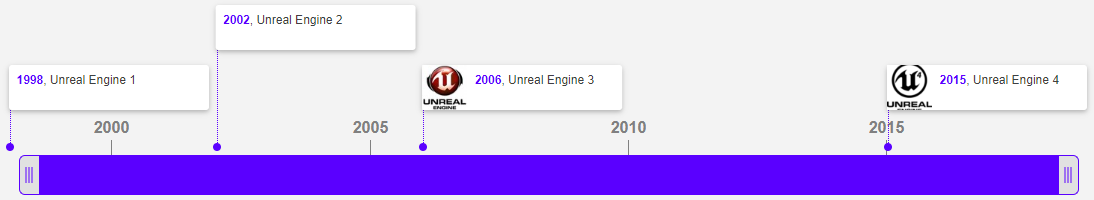
\includegraphics[width=15cm]{./images/timeline.png}
\caption{Timeline de Unreal Engine}
\end{figure}

\acs{UE4} permite portar los videojuegos a distintas plataformas, como son: PC, PlayStation 4, Xbox One, Android, iOS y Mac. Además, posee un gran soporte para dispositivos de \ac{RV}. Por esto, \acs{UE4} es uno de los motores más populares entre los desarrolladores de videojuegos. 

\acs{UE4} posee un lenguaje de \textit{scripting} visual, denominado \textit{Blueprints}. Es un método de \textit{scripting} basado en nodos haciendo que no se necesite escribir ni una sola línea de código. Este método es muy usado para realizar prototipados rápidos de niveles. En un desarrollo completo de un videojuego, se combina la facilidad de uso de \textit{Blueprints} con la potencia del lenguaje de programación C++. Dicho lenguaje, es el lenguaje de facto en la industria de los videojuegos ya que ofrece un gran rendimiento (algo esencial en cualquier videojuego) y las posibilidades con C++ quedan limitadas tan solo por el programador.

El acceso al código fuente\footnote{https://github.com/EpicGames/UnrealEngine} completo del motor de \acs{UE4} aumenta aun más las posibilidades que ofrece \cite{6}. Se puede modificar el código fuente para aumentar el rendimiento de un desarrollo en específico, se pueden introducir nuevas características al motor que no estén ofrecidas de forma oficial por Epic Games pero que sean necesarias para un desarrollo puntual. En este contexto surgen los \textit{plugins}, como un medio para lograr explotar mejor el uso del motor de videojuegos. \acs{UE4} posee un \textit{marketplace}\footnote{https://www.unrealengine.com/marketplace/store} en el que se pueden encontrar muchos \textit{plugins} tanto gratuitos como de pago. El código fuente del motor es también útil en labores de depuración del videojuego, para entender mejor las interacciones entre el código del videojuego y el código del motor.

\acs{UE4} posee muchas características que hacen que sea uno de los motores gráficos más potentes hoy en día. Posee un editor para personalizar los sistemas de partículas, una potente solución para desarrollos de \ac{RV}, un gran editor de materiales, lo que permite crear texturas en el propio motor, sin necesidad de acudir a programas de terceros. El módulo de \ac{IA} es muy potente y fácil de usar. Se pueden crear paisajes de una forma rápida y sencilla con el módulo de Terreno y Follaje. Este módulo permite crear entornos de mundo abierto gracias al uso eficiente de la memoria y al sistema \ac{LOD} que ajusta la complejidad de los objetos en función de la distancia, para priorizar el rendimiento. Las características de post-procesado en \acs{UE4}, aumentan la calidad de los resultados visuales finales en las escenas.

Los juegos multijugador \cite{7} son uno de los mercados más buscados por los jugadores de videojuegos, principalmente por la capacidad de diversión que ofrecen los mismos, al poder interactuar con otros jugadores. En un principio, los humanos tienen una capacidad de estrategia mayor que la máquina y una inteligencia artificial muy potente requiere de una gran capacidad de cómputo. El ser humano es un ser social por naturaleza, por lo que los videojuegos multijugador tienden a ser más atractivos para la mayoría de la población.

En los juegos de multijugador local, dos o más jugadores juegan en un mismo computador, por lo que el desarrollo del videojuego es prácticamente idéntico, con las únicas diferencias de un mayor soporte a dispositivos de entrada/salida y distintos puntos de vista para los distintos jugadores. En los juegos multijugador en \ac{LAN} se encuentran varias computadoras conectadas unas con otras a través de una misma red. Este es realmente el modelo más básico de videojuegos multijugador.

En los videojuegos online, los jugadores se conectan con otros a través de grandes redes, dónde los computadores se pueden encontrar geográficamente muy distantes los unos con los otros. Tradicionalmente, se usan arquitecturas basadas en el modelo cliente-servidor \cite{8} durante el desarrollo de un videojuego online debido a que es más sencillo securizar e implementar esta solución. La partida se lleva a cabo en el servidor y los clientes simplemente renderizan la partida con los datos que reciben del servidor y recogen los eventos de entrada. Hoy en día la mayoría de juegos online permiten un número relativamente pequeño de conexiones simultáneas por sesión (de 4 a 32, normalmente). Sin embargo existen los juegos de tipo multijugador masivo o \ac{MMG}, en los que cientos o miles de jugadores pueden participar en una misma sesión.

La mayor cuestión a tener en cuenta en los videojuegos online es la latencia, entendida como la cantidad de tiempo que tardan los datos del videojuego en viajar por la red. Las \ac{LAN} proporcionan características como \textit{broadcast}, una baja latencia, un gran ancho de banda y apenas pérdida de paquetes. La calidad de las conexiones de red sobre internet son muy difíciles de predecir ya que no es factible crear conexiones punto a punto para muchos clientes. Los principales problemas en videojuegos online \cite{9} son la latencia, el \textit{jitter} y un ancho de banda bajo. Puesto que el \textit{multicast} no es soportado por todos los protocolos, el ancho de banda se ve perjudicado al tener que enviar el mismo paquete una vez (como mínimo) a cada cliente conectado. Los mecanismos de predicción pueden hacer que la experiencia de juego con una latencia alta mejore, sin embargo un \textit{jitter} alto hace que el juego sea prácticamente injugable.

Desarrollar un juego multijugador online no es una tarea sencilla, ya que es uno de los tipos de juegos más difíciles de desarrollar. Hay que tener en cuenta todas estas cuestiones anteriores y muchas otras, como la relevancia de los datos (puede que ciertas zonas del mapa que no son accesibles no tengan necesidad de intercambiar información. Teniendo esta cuestión en mente, se puede disminuir considerablemente el ancho de banda usado), además de necesitar un alto conocimiento en redes y sistemas distribuidos. Sin embargo \acs{UE4} proporciona un módulo multijugador\footnote{\url{https://www.unrealengine.com/en-US/blog/getting-started-with-unreal-multiplayer-in-cpp}} que facilita mucho la tarea de desarrollar un juego online. Si dicho módulo se combina con el \ac{SDK} o Kit de Desarrollo de Software de STEAM\footnote{\url{https://wiki.unrealengine.com/Steam,_Using_the_Steam_SDK_During_Development}} se pueden crear, buscar y unirse a sesiones de una forma sencilla.

\acs{UE4} también hace esfuerzos por mejorar la experiencia de usuario cuando existe una latencia alta. Implementa técnicas sobre el componente de movimiento de los personajes que hace que el jugador no note esa alta latencia cuando se está moviendo, en un juego de tipo \acs{FPS}).

Según \cite{10}, un videojuego debe proporcionar al jugador retos de una dificultad intermedia. Los elementos que determinan el nivel de motivación del desafío son:

\newpage

\begin{itemize}
\item Los objetivos.
\item La incertidumbre del resultado.
\item La retroalimentación del desempeño.
\end{itemize}

Para que un reto sea motivante, las metas deben estar claramente definidas y organizadas en una jerarquía que relacione los objetivos a corto y a largo plazo. El resultado del juego debe ser incierto, usando niveles de dificultad variable, distintos niveles de metas, información oculta y aleatoriedad, para evitar la trivialidad y las dificultades casi imposibles. Para mantener la motivación, la retroalimentación debe ser clara, constructiva y alentadora, lo que contribuirá a la autoestima del jugador.

Sobre esta definición encajan perfectamente los videojuegos de acción, con una campaña motivada por una historia profunda, que acompañada de una dificultad acorde al jugador hacen que la experiencia de usuario sea motivante y adictiva de jugar. En este contexto nace este proyecto, un videojuego de acción en tercera persona, con una campaña cooperativa con la posibilidad de que dos jugadores de forma online la completen. Como aliciente en la motivación del usuario, se ha optado por introducir minijuegos para poder acceder a ciertas zonas del mapa de forma que no se pierde el contacto con la historia principal y se introduce una nueva mecánica de juego con el objetivo de entretener al jugador. 

Existen una gran variedad de modelos de negocio en la industria del videojuego, que utilizan las compañías para monetizar sus productos. Sin embargo, muchos de ellos suelen encajar dentro de otros, con pequeñas variaciones. Podríamos decir que desde una perspectiva general existen los siguientes modelos de negocio básicos:

\begin{itemize}
\item Modelo \textit{Pay-to-Play}. En este modelo, se compra el contenido del juego completo por una cierta cantidad y se pueden acceder a todas las características del mismo, sin ningún tipo de limitación. Es el modelo que más se usaba, hasta que otro tipo de modelos de negocio le han ido ganando territorio.
\item Modelo \textit{Free-to-Play}. Este modelo consiste en ofrecer el contenido del videojuego gratis. La monetización vendrá de las compras de objetos dentro del juego (como pueden ser objetos decorativos, \textit{skins} para los personajes o distintos camuflajes para las armas, entre otros) y por la publicidad existente en el juego.
\item Modelo \textit{Freemium}. Este modelo consiste en ofrecer gratis el contenido del videojuego, pero no la totalidad del mismo. Se accede a una parte del videojuego limitada y en el caso de querer acceder a más partes del mismo, tendrás que pagar una determinada cantidad de dinero. Este modelo tiene otras variantes como pagar inicialmente una cantidad y acceder a cierta funcionalidad del juego. Si quieres acceder a nuevas funcionalidades, nuevos mapas, etc., hay que comprarlo a parte.
\item Modelo de Suscripción. En este modelo, se paga el contenido por una determinada cantidad de tiempo, durante el cual se puede disfrutar del videojuego. Pasado este tiempo, la suscripción se cancela y habría que volver a pagar para jugar durante más tiempo.
\end{itemize}

En los últimos años, ha ganado mucha popularidad el contenido descargable o \ac{DLC}. Se trata de contenido digital exclusivo y adicional de un videojuego, que se vende por separado y posterior al lanzamiento del mismo. Se usan para alargar el tiempo de vida del videojuego, ofreciendo nuevos mapas, armas, personajes, etc. La obtención de los \ac{DLC} no tiene sentido si no se ha obtenido antes el videojuego, ya que son productos complementarios y dependientes del juego. En numerosas ocasiones, los \ac{DLC} están sujetos a controversia ya que se venden desde el día de lanzamiento del juego, por lo que el contenido del \ac{DLC} podría estar listo para la fecha de lanzamiento del juego y podría estar incluido dentro del mismo.

Un concepto novedoso pero que cada día está ganando más adeptos es el de \textit{game as a service} \cite{11}. Este modelo de negocio es complementario al \textit{software as a service} e implica que al ser un servicio, el usuario se beneficia durante un periodo de tiempo del mismo pero no le pertenece nada, el videojuego no es suyo nunca. Dentro del \textit{game as a service} podemos encontrar el modelo de suscripción comentado anteriormente. En muchos \ac{MMO} se usan suscripciones mensuales para poder disfrutar del videojuego.

Compañías como EA\footnote{https://www.ea.com} y Xbox\footnote{https://www.xbox.com} garantizan a sus suscriptores un acceso a una gran biblioteca de títulos que se ofrecen de forma digital sin limitación. El usuario tiene que descargar esos juegos en su ordenador o su consola para poder jugar. Sin embargo, para poder disfrutar de los juegos, el usuario debe seguir pagando la suscripción mensual.

Algunas compañías como PlayStation\footnote{https://www.playstation.com} o GameFly\footnote{https://www.gamefly.com} permiten que los usuarios jueguen los videojuegos que se ejecutan en servidores remotos en un dispositivo local, eliminando la necesidad de especialización en el hardware o la necesidad de computadores potentes para jugar. Esta forma de negocio se denomina \textit{cloud gaming}.













\newpage

% Sección 3: Objetivos
\pagestyle{insection}
\section{Objetivos}
\markboth{Objetivos}{}
\lettrine[lines=2,findent=2pt,nindent=3pt,loversize=0.1]{\textcolor[gray]{0.4}{E}}{n} este capítulo se van a presentar los objetivos definidos para este proyecto que se encuentra en el ámbito del \ac{CEDV}. Se va a presentar el objetivo general del proyecto, acompañado de los objetivos específicos del mismo.

\subsection{Objetivo general}

El objetivo principal del proyecto será el diseño y desarrollo de un videojuego multijugador completo. Se llevarán a cabo todas las fases, desde la concepción (que se inicia con la idea del videojuego que se quiere crear), la creación de la historia y personajes, diseño de niveles y por último la implementación en un lenguaje de programación y las pruebas.

\subsection{Objetivos específicos}

Para llevar a cabo el objetivo general será necesario completar cada uno de los siguientes objetivos específicos:

\subsubsection{Subsistema Online}

Para conseguir que la campaña del juego pueda ser disfrutada por dos jugadores en distintos dispositivos, se va a llevar a cabo la integración del videojuego con el Subsistema Online de STEAM. Como resultado, se podrá jugar al videojuego a través de Internet, sin limitación geográfica.

\subsubsection{Diseño de Escenarios y Mecánicas de juego}

Es necesario conseguir unos escenarios atractivos visualmente y acordes a la historia para alcanzar la mayor inmersión posible en el juego por parte del jugador. De igual forma, las mecánicas de juego deben coincidir con el tipo de juego planteado y la historia del mismo, para dar el mayor sentido posible al videojuego.

\subsubsection{Diseño e Implementación del Minijuego}

Para añadir una jugabilidad extra que dote al juego de más contenido y permita al jugador relajarse, se introducirá en el juego una forma para acceder a ciertos lugares, basada en la resolución de un puzzle. 

\subsubsection{Personajes del videojuego e \ac{IA}}

Se diseñarán y codificarán todos los personajes que van a aparecer en el juego, tanto aliados como enemigos. Se va a diseñar la \ac{IA} correspondiente de cada uno, dotándoles de un comportamiento aparentemente inteligente para ofrecer una mayor sensación de inmersión al jugador. Los personajes serán capaces de identificar al jugador, moverse hacia él y atacarle, si se encuentran a una distancia propicia para ello.

\pagestyle{notsection}

\subsubsection{Diseño de la \ac{GUI}}

Se procederá a realizar un diseño de la interfaz gráfica del juego, interfaz de diálogos y distintos menús que conforman \textit{Alliance}, que sea agradable para el jugador y que concorde con la temática del videojuego. Con esto, se pretende maximizar el objetivo de todo videojuego, el entretenimiento.
\newpage

% Sección 4: Arquitectura de la solución
\pagestyle{insection}
\section{Arquitectura de la solución}
\markboth{Arquitectura de la solución}{}
\subsection{Diseño de personajes}
Para nuestro juego, y puesto que ninguno de los desarrolladores que hemos trabajado en este proyecto tenemos ninguna experiencia en la creación y diseño gráfico de personajes, animaciones, o cualquier otro tipo de \textit{asset} requerido en este proyecto, hemos decidido utilizar los \textit{assets} que se liberaron recientemente del videojuego de \textit{Epic Games} llamado \textit{Paragon}\footnote{Juego que, por otra parte, ha cerrado todos sus servidores.}.
\\

Puesto que nuestros modelos son todos importados (y, en el caso de los modelos de los personajes, de \textit{Paragon}), tenemos modelos y decorados con un acabado más profesional del que nosotros podríamos haber conseguido. Sin embargo esta situación crea un problema: Nos encontramos limitados a lo hora de hacer nuestro sistema de combate. Las animaciones de ataque de los esqueletos ya vienen definidas, y tenemos que intentar amoldarnos a lo que nos viene hecho. Ni siquiera podíamos usar software externo para crear nuevas animaciones, porque estos modelos se importan directamente al proyecto.
\\

Dicho esto, podemos empezar a explicar la solución que hemos adoptado para modelar a los personajes.

\subsubsection{Diseño de los personajes aliados}

\begin{figure}[H]
  \centering
  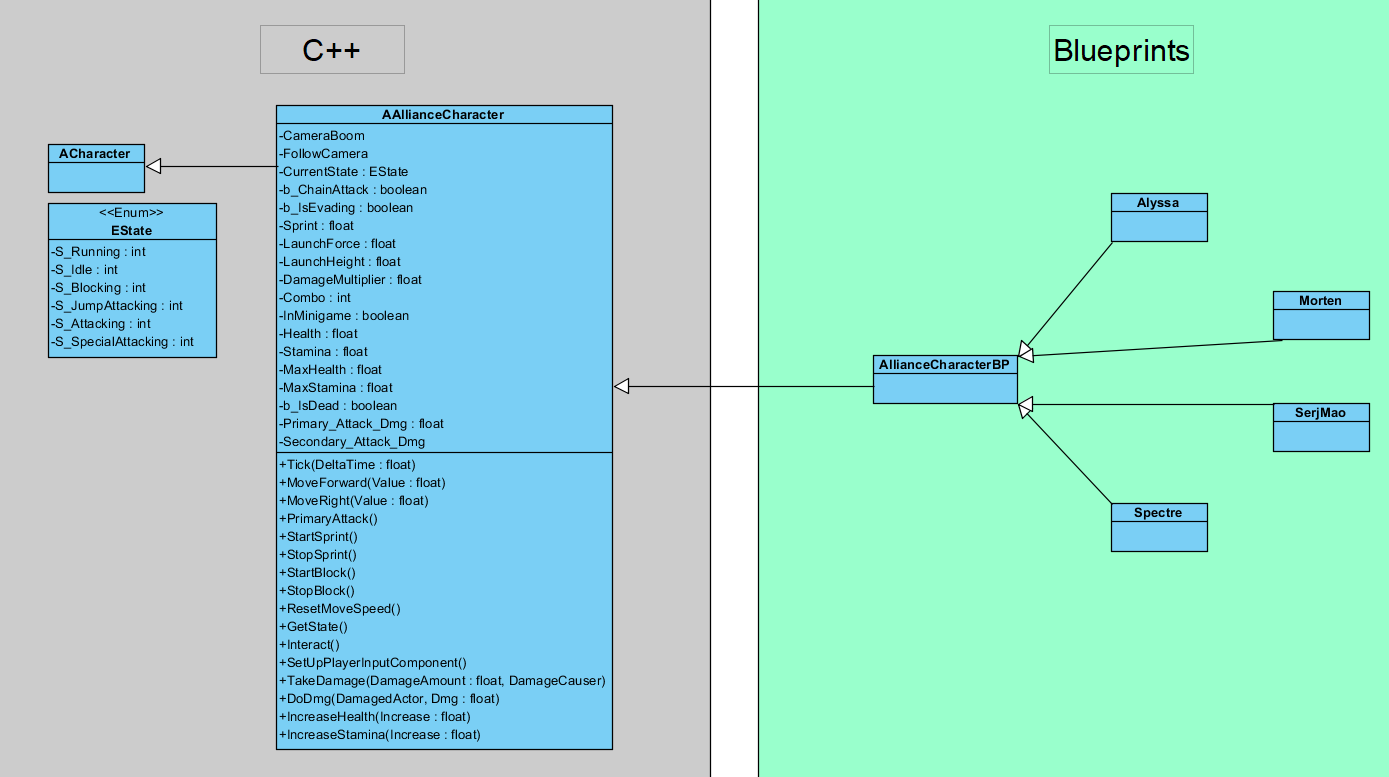
\includegraphics[width=10cm]{./images/Classes_Aliados.png}
  \caption{Fragmento del diagrama de clases relacionado con los personajes aliados}
  \label{ClassesAllies}
\end{figure}

En el diagrama se puede ver cómo se ha optado por hacer una clase base en C++, \texttt{\textbf{AAllianceCharacter}}. Esta clase contiene toda la funcionalidad básica de un personaje, ya sea controlado por inteligencia artificial o por el jugador. Esta funcionalidad básica se puede resumir en todas las propiedades necesarias (Vida, estamina, daño, etc), aunque la mayoría de estas propiedades no serán inicializadas en el constructor de esta clase. Esta clase está pensada para que no haya ninguna instancia de ella en el mundo, por eso no contiene ningún componente típico de los actores que van a ser representados en él, como por ejemplo el esqueleto.
\\

En esta clase base se pueden resaltar ciertos aspectos importantes:
\begin{itemize}
\item La clase sirve también para dar la funcionalidad base de la replicación en red (de la que se hablará más adelante)
\item Debido al punto anterior, muchos de los métodos de que se pueden ver en el diagrama de clases están duplicados, para el cliente y el servidor.
\item Muchas de las variables de clase ni siquiera son usadas en esta clase, si no que sirven para las clases que modelan personajes del juego.
\item El método Tick nos da la funcionalidad de regeneración de vida y estamina.
\item Los métodos de \texttt{DoDmg()} y \texttt{TakeDamage()} llaman a los eventos internos de \ac{UE4} para causar daño, que hemos sobrescrito nosotros.
\end{itemize}


Hablaremos más adelante de la máquina de estados que esta clase tiene cuando hablemos del \textbf{sistema de combate}.
\\

Una vez discutida la clase \textbf{AAllianceCharacter}, también se puede ver que tenemos una clase base más, esta vez en \ac{BP}. La clase base en \ac{BP} sirve para modelar cierta funcionalidad básica que necesitamos que sea en Blueprints, como ciertos widgets de la \ac{GUI} o cierta parte de replicación (discutida más adelante). También nos sirve para especificar algunos componentes de los personajes, como el componente de movimiento.
\\

Todas las clases de los personajes del juego están hechas en \ac{BP}. Prácticamente toda la responsabilidad de estas clases es la de modelar el sistema de combate de cada personaje (El cuál se discutirá más adelante). Esto es gracias a que toda la funcionalidad extra (Replicación, comunicación con otros blueprints en caso de, por ejemplo, causar daño, etc) ya está definida en las clases mencionadas anteriormente. Estas clases se han modelado en \ac{BP} por las numerosas ventajas que proporciona: La posibilidad de ajustar el \textit{Skeletal Mesh} directamente en el editor, facilidad para añadir componentes en \textit{sockets} específicos de forma visual (Se hablará más adelante de esto), y ,lo que más importante nos ha parecido, la posibilidad de elegir un \textit{asset} directamente desde un menú desplegable al cambiar el valor de una variable, entre otras. Obviamente, el hecho de modelar estos comportamientos un poco más complejos en \ac{BP} conlleva ciertas desventajas, entre las que hemos encontrado la baja mantenibilidad, y la mala capacidad para compartir el trabajo, porque los Blueprints son archivos binarios.
\\

También es importante recalcar que casi todas las propiedades son inicializadas en el constructor de estas clases, porque cada personaje tendrá sus propios valores de vida, estamina, daño, etc. A continuación un ejemplo:

\begin{figure}[H]
  \centering
  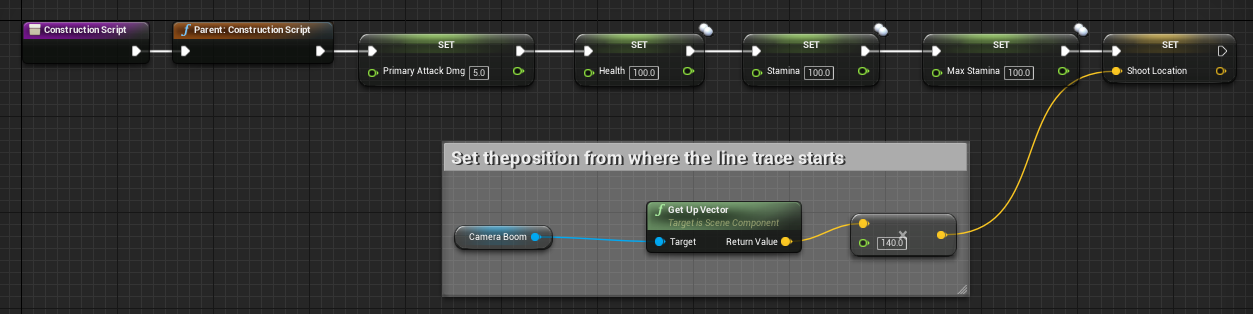
\includegraphics[width=10cm]{./images/BP_Morten_Constructor.png}
  \caption{Constructor para la clase Morten}
  \label{MortenConstructor}
\end{figure}


\subsubsection{Diseño de personajes enemigos}

\begin{figure}[H]
  \centering
  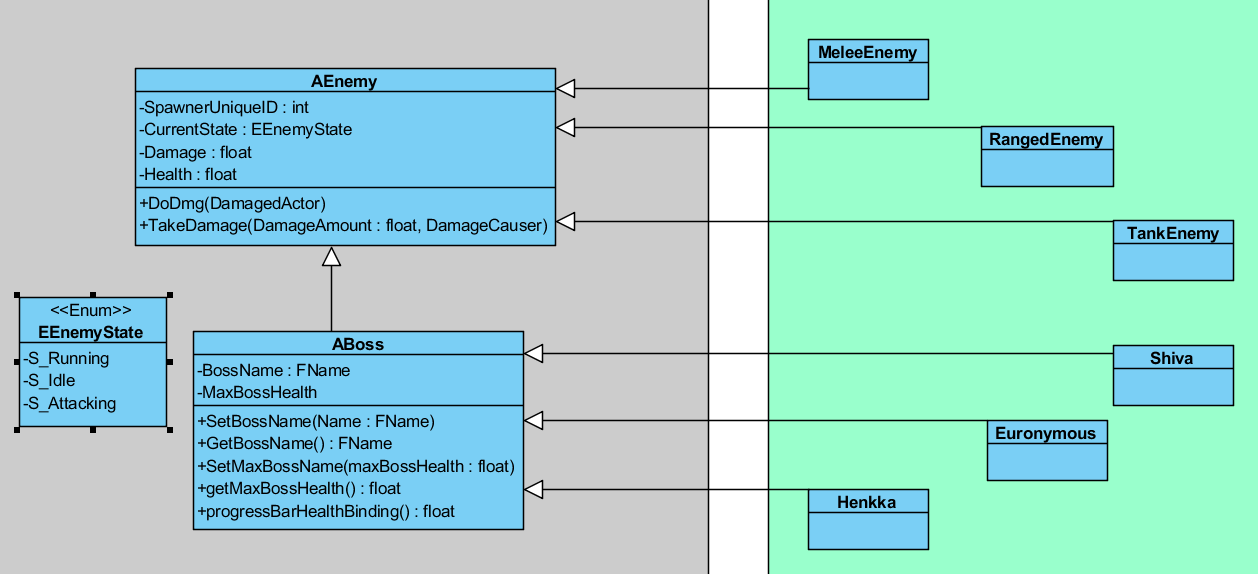
\includegraphics[width=10cm]{./images/Classes_Enemigos.png}
  \caption{Fragmento del diagrama de clases relacionado con los personajes enemigos}
  \label{ClassesEnemies}
\end{figure}

Se puede observar como la solución es muy similar al diseño de los personajes aliados: una clase base en C++ con la funcionalidad necesaria, y extensión en \ac{BP} para las clases particulares de cada enemigo. Esto es porque valoramos más las ventajas frente a las desventajas que hemos discutido anteriormente en esta sección también. Igualmente, se hablará de la máquina de estados de los enemigos en la sección del \textbf{sistema de combate}.
\\

En este caso, hemos decidido crear una clase base más para el caso particular de los jefes de zona (\textit{Bosses}). Esto es porque los jefes tienen ciertas funcionalidades comunes pero que son básicas, como por ejemplo las barras de vida.
\\

Al igual que con los aliados, la mayoría de las propiedades son inicializadas en el constructor de la clase en \ac{BP}, por el mismo motivo, cada enemigo tendrá sus propios valores de vida, daño, etc.

\subsection{Diseño del minijuego}
El diseño del minijuego está dividido en dos clases, \textit{Board} y \textit{Piece}, la primera es la encargada de saber la posición de todas las piezas, comprobar los movimientos válidos de cada pieza y saber cuándo se ha ganado el juego. La segunda, por el contrario únicamente conoce su posición actual y sus dimensiones, también se encargará de ejecutar la \textit{Timeline} que la moverá a la casilla que se le indique. \\

\subsubsection{Representación del minijuego}
Para la representación del tablero se ha usado la estructura de datos \textit{TBitArray}. Se ha escogido esta estructura de datos debido a su bajo tamaño en memoria. En este array se guarda qué celdas están ocupadas y cuáles no. \\

Complementario a este, existe otro array de piezas, el cual se usa para cambiar que pieza está seleccionada, mover las piezas y comprobar si un movimiento es válido. Ninguno de estos dos arrays está replicado ya que estos se actualizan con las llamadas \ac{RPC} que permiten mover las piezas. \\

A parte de estas dos propiedades el tablero también tiene una serie de delegados para notificar de una serie de eventos: \\

\begin{itemize}
	\item \textbf{OnMiniGameFinished}: Informa de que el minijuego ha acabado para, por ejemplo, ocultar la interfaz del minijuego, abrir la puerta y ejecutar la animación de la cámara.
	\item \textbf{OnChangePieceToSelected}: Informa de que el jugador que está en el servidor ha cambiado la pieza seleccionada al jugador que está en el cliente para que este también cambie la pieza seleccionada.
	\item \textbf{OnChangePieceToItsColor}: Informa de que el color de la pieza indicada ha cambiado de color, indicandole al cliente de que también cambie el color a esa pieza.
	\item \textbf{OnMovePiece}: Informa de que la pieza indicada se está moviendo para que el cliente ejecute también la \textit{timeline} asociada a la pieza.
\end{itemize} \\

Para la representación de las piezas se ha optado por guardar únicamente su tamaño y su posición (de la esquina superior izquierda). Estos valores se pueden editar dentro del editor para así poder ajustar la dificultad del minijuego de una forma más sencilla comparado con editar los valores en C++/Blueprints.\\


\subsubsection{Reproducción del minijuego en pantalla}

Durante el diseño del juego se consideraron dos formas de mostrar el minijuego al jugador, la primera opción pasaría por colocar todos los actores del minijuego en la misma localización donde se mostrarían durante la partida, la segunda consistiría en colocar el minijuego en un lugar del nivel donde no se pudiese ver por el jugador durante el gameplay normal y posteriormente, por medio de una \textit{Scene Capture 2D} mostrarsela al jugador como si de una pantalla se tratase.

La primera opción se descartó debido a los siguientes problemas:

\begin{itemize}
	\item La gran cantidad de actores que se necesitan para mostrar el minijuego aumentaba la dificultad de mostrar/ocultar el minijuego.
	\item La dificultad de crear nuevos minijuegos en localizaciones distintas debido a la gran cantidad de actores que posicionar correctamente.
	\item La poca flexibilidad en términos de tamaños, si se quiere ajustar el minijuego a una puerta más pequeña se tendrían que escalar todo el tablero.
\end{itemize}

Por lo que la segunda opción fue la desarrollada, esta opción cuenta con la ventaja de que da una sensación de inmersión con la temática de la historia planteada. Esta opción está formada por tres componentes que se describirán a continuación:

\paragraph{Disposición del minijuego en el nivel}

Todos los minijuegos están colocados en una caja debajo del suelo de cada nivel para que el jugador no pueda encontrarselos en un gameplay normal. Una gran ventaja de este enfoque es la capacidad de crear nuevos minijuegos a partir de los anteriores, únicamente con copiar todos los contenidos de una caja en otra posición del nivel se crea un nuevo minijuego, solo haría falta colocar una nueva pantalla en el nivel. \\

\begin{figure}[H]
  \centering
  \includegraphics[width=13cm]{./images/Minigame_When_Playing2.png}
  \caption{Contenido dentro de la caja del minijuego durante el gameplay}
  \label{MinigameWhenPlaying}
\end{figure}

\paragraph{\textit{Scene Capture 2D} para mostrar en minijuego en una "pantalla"}
Para mostrar el minijuego en otra parte del nivel se recurrió a una \textit{Scene Capture}, concretamente a un \textit{Scene Capture 2D}. Este actor actúa como si de una cámara se tratase solo que esta en vez de mostrar lo que captura a través de la pantalla del jugador guarda la imagen en una textura para su posterior uso en un material el cual se usa en un plano para mostrarlo dentro del nivel.

\begin{figure}[H]
  \centering
  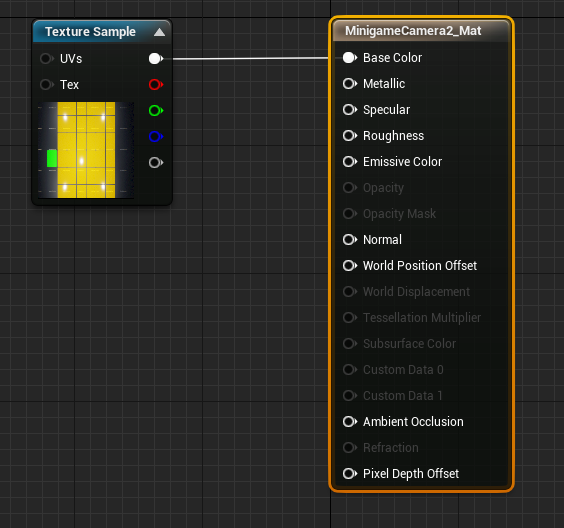
\includegraphics[width=11cm]{./images/Screen_Capture_To_Mat.png}
  \caption{Material para mostrar el \textit{Scene Capture 2D}}
  \label{SceneCapture2DMat}
\end{figure}


\begin{figure}[H]
  \centering
  \includegraphics[width=14cm]{./images/Minigame_When_Playing.png}
  \caption{Plano del minijuego durante el gameplay}
  \label{GameplayMinigame}
\end{figure}

\paragraph{Blueprint que maneja el gameplay del minijuego}
Para la interacción inicial con el minijuego y las tareas de movimiento de la cámara, apertura de puertas y gestión de la intefaz se ha creado una clase \textit{Blueprint} que hereda de \textit{Trigger Box}, el \textit{MinigameStarter\_Blueprint} .Para realizar todas estas tareas este se suscribe a los delegados del \textit{Board} que se comentaron anteriormente, demostrando una forma de comunicación entre C++ y Blueprints. \\

Para sugerir al jugador de que puede interactuar con este actor se han añadido tanto un sistema de partículas que se activa cuando el minijuego está disponible para ser jugado como un texto que aparece cuando el jugador pasa por encima de este actor dando, de esta forma, información de que el jugador puede interactuar sin ser intrusivo, como podría ser un diálogo o un tutorial.


\begin{figure}[H]
  \centering
  \includegraphics[width=14cm]{./images/Minigame_Press_Play.png}
  \caption{Interacción con el \textit{MinigameStarter_Blueprint}}
  \label{Minigamestarterinteraction}
\end{figure}

\subsection{Sistema de combate}
El sistema de combate en un juego de este estilo acaba resultando la mayor parte de la experiencia de juego. Por eso, es necesario hacer un incapié especial en él.
En nuestro caso, hemos decidido crear dos personajes principales: Alyssa Y Morten. Cada uno de ellos tiene armas distintas y por tanto, la forma de combatir es treméndamente distinto: Alyssa combate cuerpo a cuerpo, mientras que Morten ataca a distancia. Esto provoca que la elección de personaje antes del inicio del juego sea más interesante, y que además, en el caso de jugar en modo multijugador, se genera una mayor distinción entre los roles de cada jugador. 
\\

A la hora de diseñar los distintos ataques que cada jugador podría hacer, era importante tener en cuenta las animaciones que teníamos, porque, como ya se ha dicho antes, nos encontrábamos muy limitados. Aún así, hemos conseguido hacer que cada personaje, aliado o enemigo, tenga un ataque principal basado en un combo de varios golpes (En el caso de los que atacan en combate cuerpo a cuerpo). Además, los personajes principales pueden esprintar, bloquear, esquivar, y tienen un ataque especial.
En el caso particular de Alyssa también puede atacar en carrera y tiene otro ataque especial más. 
\\

Un problema en cuanto a diseño de mecánicas es que los jugadores podrían <<abusar>> de los ataques especiales (que causan más daño), además del esquive o el sprint. Para limitar las posibilidades del jugador y evitar que el juego resulte extremadamente sencillo, se ha optado por implementar un sistema de estamina, que se regenera mucho mas rápido que la salud, pero los ataques especiales consumen gran parte del total. Aún así, es importante mantener la regeneración a un nivel más o menos alto, para evitar que el jugador se encuentre sin posibilidades de actuación; en resumen, es un sistema muy difícil de balancear. 
\\

Prácticamente todo el sistema de combate (Salvo los eventos de causar y recibir daño) está modelado en \ac{BP}. Este sistema consta de varias partes importantes que vamos a discutir a continuación: Las máquinas de estados que tienen todos los personajes, y la comunicación entre los Blueprints de cada personaje.
\\

Para los personajes que atacan cuerpo a cuerpo, se ha optado por añadir unas cápsulas de colisión en las armas, que son añadidas a un \textit{socket} (Normalmente el de la mano) para que se muevan acorde a las animaciones del personaje. Estos componentes serán los encargados de detectar la colisión con un enemigo. Usar este tipo de sistema conlleva una serie de problemas, cuya solución discutiremos más adelante. A continuación una foto de cómo estas cápsulas son añadidas a un personaje.


\begin{figure}[H]
  \centering
  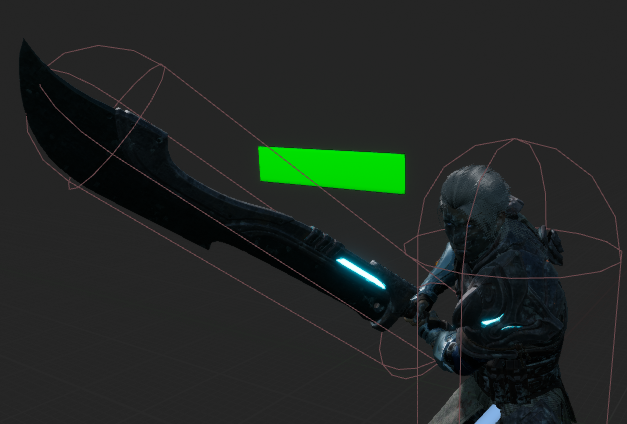
\includegraphics[width=10cm]{./images/Eur_Weapon.png}
  \caption{Cápsulas de colisión en la espada de Euronymous}
  \label{HenkkaSM}
\end{figure}


\subsubsection{Comunicación entre Blueprints}

Todos los personajes tienen asociado un Blueprint de animación o \ac{ABP}. Este Blueprint tiene, en nuestro proyecto, dos finalidades importantes:


\begin{itemize}
\item[1] Definir el Blendspace a usar. Un Blendspace es una combinación de dos o más animaciones, que \ac{UE4} es capaz de combinar en base a cierto valor. En nuestro caso, combinamos la animación de estar parado (o Idle) con la de moverse. En el caso de los personajes jugables, puesto que pueden esprintar, también se combinaría con la animación de correr. El \ac{ABP} es el encargado de comunicar el valor de velocidad al Blendspace. Este Blendspace también puede ser cambiado en cualquier momento desde el \ac{ABP}, que se controla mediante una máquina de estados, aunque esto sólo se ha hecho con un personaje en particular. A continuación este caso.


\begin{figure}[H]
  \centering
  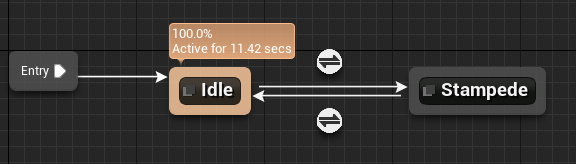
\includegraphics[width=10cm]{./images/Henkka_SM.png}
  \caption{Máquina de estados de los Blendspaces de Henkka}
  \label{HenkkaSM}
\end{figure}


Las transiciones entre un Blendspace u otro también son responsabilidad del \ac{ABP}, aunque lo que éste hace es comprobar una variable de la clase en \ac{BP}.

\item[2] Controlar la comunicación entre el \ac{BP} y el \ac{ABP}. Esto vamos a ampliarlo a continuación.
\end{itemize}


A la hora de modelar el \textbf{sistema de combate}, nos encontramos con la problemática de las animaciones. Una vez ya teníamos modeladas las animaciones <<constantes>>, es decir, las que mantiene el personaje si no realiza ninguna acción (La animación de movimiento o la de sprint), tuvimos que modelar las animaciones de ataque. La solución que adoptamos consiste en convertir las animaciones en los denominados \textit{Animation Montage}. Estos montajes nos permiten añadir notificaciones en momentos determinados de cada animación. Ésta es la base de toda nuestra comunicación entre Blueprints.
\\

El flujo que seguimos a la hora de realizar un ataque es el siguiente:

\begin{itemize}
\item[1] El jugador o el controlador de inteligencia artificial llaman al evento asociado de un ataque en concreto.
\item[2] El flujo de ejecución del evento hace que el personaje realice una determinada animación.
\item[3] La animación genera numerosos eventos a lo largo de su ejecución, pudiendo estos eventos cambiar el estado del personaje, o generar la ejecución de nuevas animaciones.
\end{itemize}


A continuación se ilustra este flujo de ejecución con un diagrama de secuencia para un caso concreto: El ataque en carrera de Alyssa.


\begin{figure}[H]
  \centering
  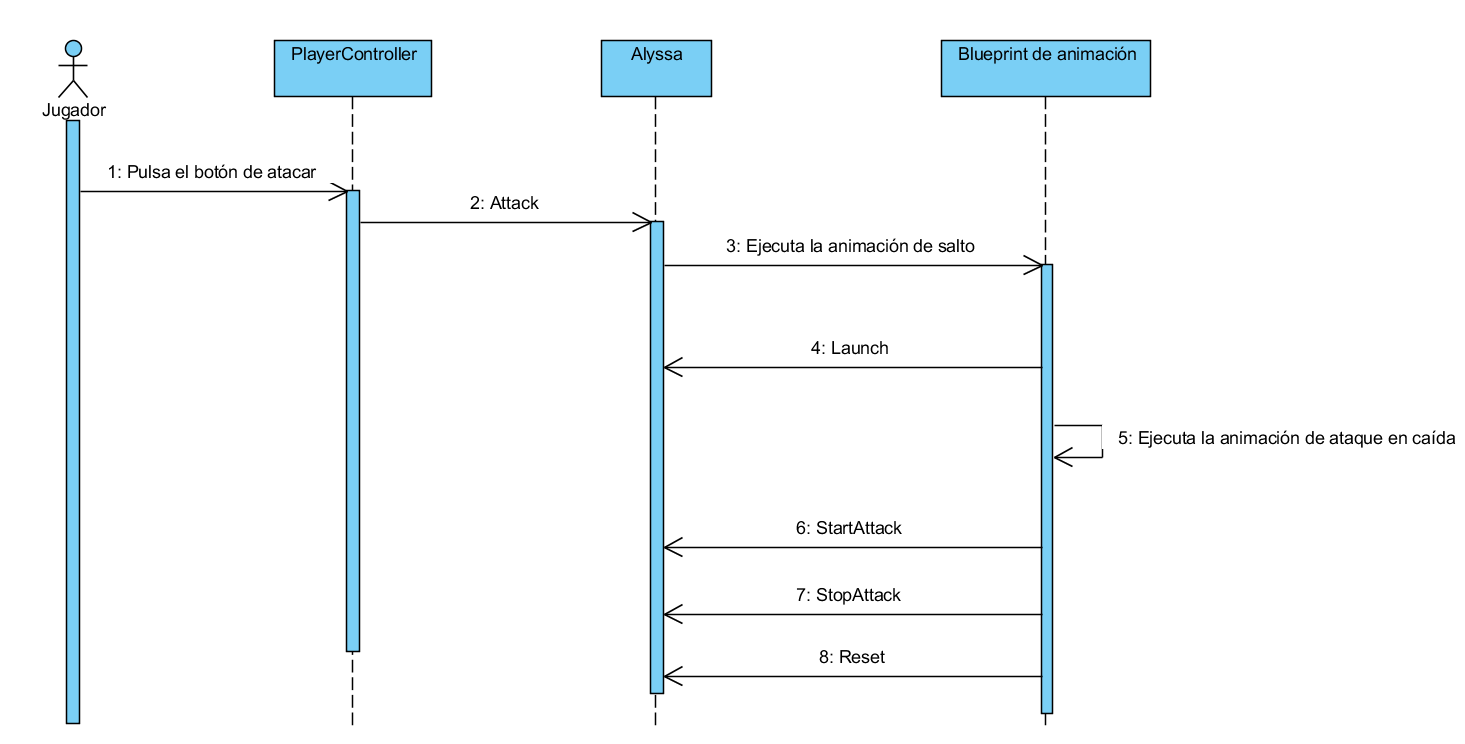
\includegraphics[width=10cm]{./images/Secuencia_Alyssa.png}
  \caption{Diagrama de secuencia para el ataque en salto de Alyssa}
  \label{AlyssaS}
\end{figure}


Es importante recalcar que el Blueprint de animación no es el encargado de ejecutar las animaciones, pero se ha escrito así en el diagrama por motivos descriptivos. En el diagrama \ref{AlyssaS} se puede ver cómo el \ac{ABP} se comunica con la clase Blueprints para cambiar su estado y lanzar nuevas animaciones. En el caso concreto anterior, \textit{Launch} es un evento que empuja al personaje hacia delante, recreando la sensación de salto en carrera. Los eventos de \textit{StartAttack} y \textit{StopAttack} los comentaremos más adelante.


Para ilustrar mejor cómo funciona esta comunicación, adjuntamos capturas de un \textit{Animantion Montage} cualquiera y de cómo se llaman los eventos en el \ac{ABP}.

\begin{figure}[H]
  \centering
  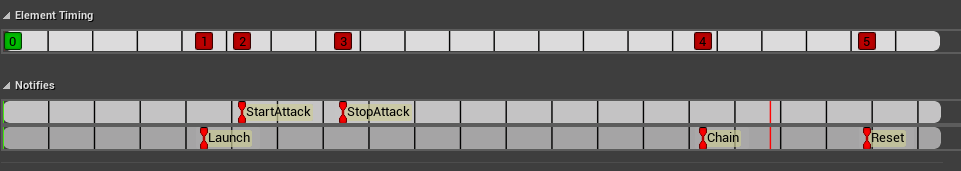
\includegraphics[width=10cm]{./images/Notifs_Montage.png}
  \caption{Barra de notificaciones de un Animation Montage}
  \label{AlyssaM}
\end{figure}


\begin{figure}[H]
  \centering
  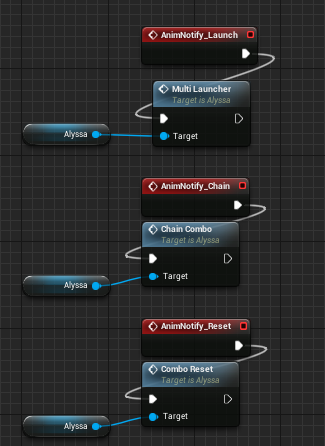
\includegraphics[width=10cm]{./images/Notifs_ABP.png}
  \caption{Comunicación entre las notificaciones de los montajes y la clase de Alyssa}
  \label{AlyssaABP}
\end{figure}


En la figura \ref{AlyssaM} Se puede ver una barra de notificaciones de un montaje. Ahí podemos poner las notificaciones que queramos en el instante de cada animación que queramos. Estas notificaciones generan eventos en el \ac{ABP} asociado, y como se puede ver en la Figura \ref{AlyssaABP}, desde estos eventos llamamos a las funciones de la clase de Blueprints.
\\

Gracias a esta comunicación, hemos podido modelar comportamientos más precisos de lo que en un principio se habían considerado. Un caso específico es la detección de colisiones. Como veremos más tarde, cada personaje tiene una máquina de estados asociada. Sin embargo, comprobar si el estado de un personaje es \textit{atacando} no es suficiente para evitar problemas, como que la cápsula de colisión haga \textit{overlap} con el enemigo varias veces, o que el enemigo colisione con ella justo antes de que la animación termine y no tiene sentido que se produzca daño, o incluso, para los enemigos de dos armas, que se haga \textit{overlap} con el arma que no está atacando. Para hacerlo más preciso, se ha optado por utilizar las notificaciones mencionadas antes para notificar exactamente cuándo y qué arma tiene que empezar a hacer daño, y cuando tiene que parar. Ésto se puede ver tanto en la Figura \ref{AlyssaS}, donde se explica que en el ataque en salto se llaman a esas dos funciones, como en la Figura \ref{AlyssaM}, donde se ven dichas notificaciones en la barra de notificaciones del montaje.

\subsubsection{Estados de los personajes}

Al modelar el \textbf{sistema de combate} y trabajar con animaciones, surgen problemas importantes, como evitar que el jugador se mueva mientras está atacando, evitar que dos animaciones no se solapen cuando no deban, y a la hora de tratar con controladores de inteligencia artificial (que mandan ordenes mucho más rápido que un humano en ciertas ocasiones), evitar que algunas acciones queden <<sepultadas>>. Una primera opción que se consideró en la etapa de prototipado fue la inclusión de varias flags o valores \textit{booleanos}, pero a medida que añadiamos funcionalidad a los personajes, se hacía claro que necesitábamos un mejor diseño. La solución obvia era la inclusión de estados en cada uno de los personajes. En las figuras \ref{ClassesAllies} y \ref{ClassesEnemies} se pueden ver los estados (Implementados mediante enumeraciones) para los aliados y los enemigos. A continuación también incluimos unas máquinas de estados para ilustrar los cambios que pueden suceder.


\begin{figure}[H]
  \centering
  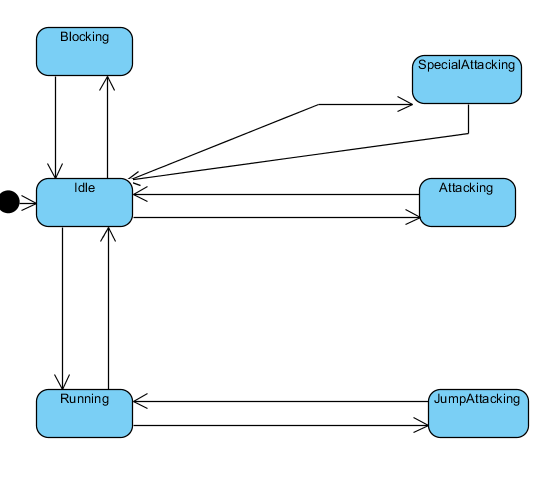
\includegraphics[width=10cm]{./images/SM_Ally.png}
  \caption{Máquina de estados para los personajes aliados}
  \label{AllySM}
\end{figure}

\begin{figure}[H]
  \centering
  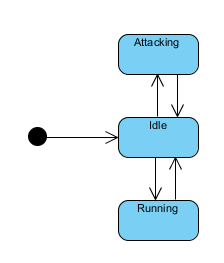
\includegraphics[width=10cm]{./images/SM_Enemy.png}
  \caption{Máquina de estados para los personajes aliados}
  \label{EnemySM}
\end{figure}


También hay que tener presente que, los personajes aliados que no son jugables, no van a llegar nunca a los estados como SpecialAttacking.


Con este sistema, es importante controlar de forma correcta los cambios de estado en cualquier momento. Esto es especialmente importante en los controladores de inteligencia artificial, donde las acciones pueden ser bastante más rápidas de ejecutar (esto es, el controlador puede ser que llame a varias funciones de forma muy seguida, aunque luego el personaje las ejecute a una velocidad más natural). Dado que el estado es controlado de forma correcta, podemos comprobar fácilmente si un personaje debería moverse o no en un instante, o si puede atacar o no en un momento dado. A continuación algunos ejemplos de cómo se controla.


\begin{figure}[H]
  \centering
  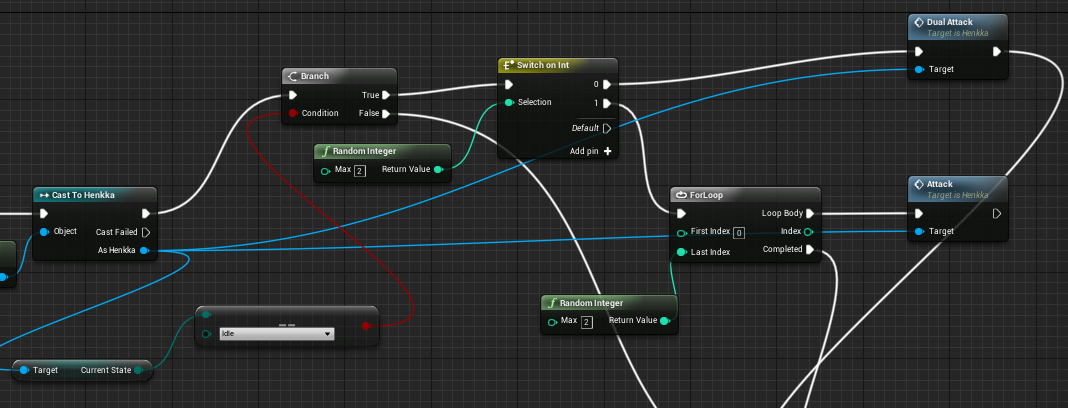
\includegraphics[width=10cm]{./images/Henkka_Attack.png}
  \caption{Ataque de uno de los jefes}
  \label{HenkkaAttack}
\end{figure}

\begin{figure}[H]
  \centering
  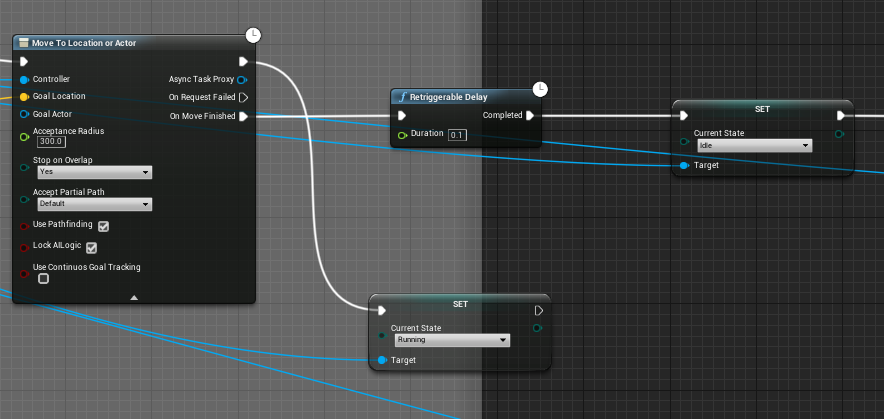
\includegraphics[width=10cm]{./images/Henkka_Move.png}
  \caption{Movimiento de un personaje controlado por IA}
  \label{HenkkaMove}
\end{figure}


en la Figura \ref{HenkkaAttack} se puede ver como podemos controlar si un personaje debería poder atacar en un instante determinado, si el personaje no se está moviendo o no está atacando. En la Figura \ref{HenkkaMove} podemos ver algo parecido. Cuando un personaje (En este caso controlado por \ac{IA}) empieza a moverse, se cambia el estado a \textit{Running}. Cuando el movimiento acaba (En este caso, el flujo de ejecución empieza en el pin \textit{OnMoveFinished}), volvemos a poner el estado a \textit{Idle}.
\\

Este sistema de estados también nos permite funcionalidades muy interesantes, como la función \texttt{ResetSpeed()}, que nos resetea la velocidad dependiendo del estado después de modificarla de alguna manera.

\begin{lstlisting}[language=c++,caption={},captionpos=b,label={ResetSpeed}]
void AAllianceCharacter::ResetSpeed_Implementation()
{
	if (!InMinigame)
	{
		switch (CurrentState)
		{
		case EState::S_Idle:
			GetCharacterMovement()->MaxWalkSpeed = 1200.f;
			break;
		case EState::S_Running:
			GetCharacterMovement()->MaxWalkSpeed = 1200.f + Sprint;
			break;
		case EState::S_Blocking:
			GetCharacterMovement()->MaxWalkSpeed = 600.f;
			break;
		default:
			GetCharacterMovement()->MaxWalkSpeed = 1200.f;
			break;
		}
	}
}
\end{lstlisting}


\subsubsection{Inteligencia Artificial}

Una parte muy importante de un sistema de combate es la inteligencia artificial de los enemigos. Los enemigos en este proyecto se han separado en dos grandes grupos: Enemigos básicos, y jefes finales. A su vez, hay 3 tipos de enemigos básicos, y 3 jefes finales diferentes. Por eso, cada uno tendrá una inteligencia artificial ligeramente distinta a las de otros enemigos.
\\

La inteligencia artificial de todos los personajes en \textit{Alliance} se basa en el sentido de la vista. Todos los personajes controlados por inteligencia artificial se rigen por este sentido, siendo capaces de ver otros personajes en su rango de visión y siendo capaces de distinguir si son aliados o enemigos. En caso de que detecten un enemigo, lo guardan en memoria como \textit{Aggro}, y empiezan a perseguirlo. Aquí aparecen los dos problemas que hemos tenido a la hora de diseñar la \ac{IA} en nuestro proyecto. El primero es que, por algún motivo, los enemigos <<miran>> por su derecha. El cono de visión tiene su centro en un ángulo de menos 90 grados con respecto a su vector frontal, y no hemos sido capaces de solucionarlo. El segundo problema que nos hemos encontrado resulta del uso de la función \textit{MoveTo} en las tareas de los árboles de comportamiento. Éste nodo mueve al personaje hacia donde está su objetivo en el momento de llamarlo, pero por algún motivo, y por cómo se ha diseñado la tarea de movimiento, no parece seguir a su objetivo, si no que se mueve hacia ese lugar. Esto resulta en un comportamiento un poco menos inteligente del esperado.
\\

Pasamos ahora a presentar un ejemplo de un árbol de comportamiento de un enemigo básico. 

\begin{figure}[H]
  \centering
  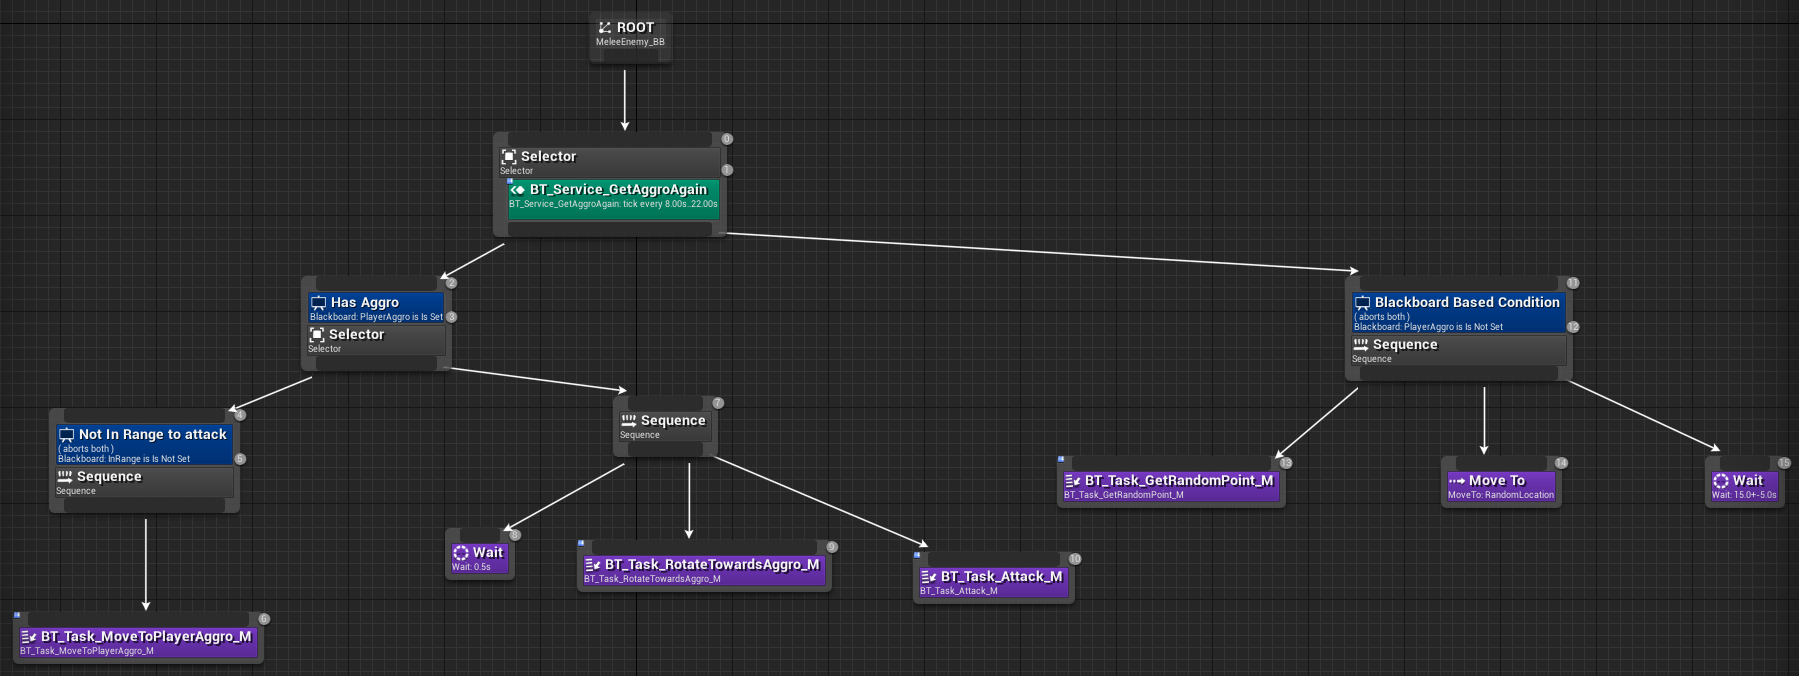
\includegraphics[width=10cm]{./images/BT_Basic.png}
  \caption{Árbol de comportamiento para un enemigo cuerpo a cuerpo}
  \label{BTBasic}
\end{figure}


En la Figura \ref{BTBasic} se puede ver como, el enemigo seguirá al personaje que tenga \textit{Aggro}, y si está a rango de atacar, atacará. También se moverá a un lugar cercano aleatorio en caso de que no vea a ningún enemigo. El servicio \textit{GetAggroAgain} sirve para evitar posibles bloqueos, que se pueden dar de forma extremadamente rara cuando el \textit{Aggro} muere en el instante que va desde el inicio de la tarea \textit{MoveToPlayerAggro} y el momento en que esa tarea llama a la función \textit{MoveTo}. Este suceso puede pasar sobre todo en la inteligencia artificial de los aliados no jugables, pero sucede de forma extremadamente rara (Tan rara que hemos sido incapaces de replicar ese error en un entorno controlado, y no hemos podido testearlo). El servicio \textit{GetAggroAgain} también cambia el objetivo de ataque, resultando en que un enemigo (O jefe) no te seguirá continuamente. Este servicio no sucede de forma muy frecuente, y muchos enemigos básicos ni siquiera tienen tiempo de llamarlo.
\\

La mayor diferencia entre cada tipo de enemigo básico no está en el árbol de comportamiento, si no en las tareas en sí. Obviamente no tiene sentido que un enemigo que ataca a distancia te siga de cerca. Aún así las diferencias entre los enemigos básicos no son demasiadas.
\\

La inteligencia artificial de los aliados controlados por un controlador de {IA} es similar a la de los enemigos básicos. Al igual que los enemigos a distancia, Morten tampoco sigue a los enemigos de cerca, si no que los ataca en cuanto está a rango. Los otros dos (Alyssa y Serj Mao) sí que siguen a los enemigos de cerca y los atacan si están a rango, y también pueden cambiar de objetivo cada cierto tiempo. También tienen otro servicio, \textit{CheckForEnemies}, para comprobar si sigue habiendo enemigos cercanos al matar a su objetivo. Cuando no están en batalla, siguen al jugador de cerca.
\\

El caso de los jefes finales es el más complejo. En realidad, la base del árbol de comportamiento es la misma: Esperan a ver a un personaje a quien puedan atacar, y si lo ven, lo persiguen y lo atacan si están a rango. Sin embargo, los jefes tienen varios tipos distintos de ataque básico, que en todos los casos es elegido de forma aleatoria. Además, cada jefe tiene una particularidad única, y esto se ve reflejado en su árbol de comportamiento:

\begin{itemize}
\item Henkka empezará a perseguir en carrera y atacar rápidamente cuando está bajo de vida.
\item Euronymous Tiene una probabilidad de <<mejorarse>>, ganando la habilidad de atacar a distancia durante diez segundos con sus ataques básicos (Simulando que es capaz de cortar el viento). Cuando está bajo de vida, esta probabilidad se eleva. Cuando se <<mejora>>, hace una animación especial para que el jugador se entere.
\item Shiva Tiene una probabilidad, que al igual que Euronymous aumenta cuando está bajo de vida, de hacer más daño durante unos momentos.
\end{itemize}

Además, por motivos de historia del juego, Shiva se regenera muchísima salud al principio del combate.


Por estos motivos, Los árboles de comportamiento para cada jefe son ligeramente diferentes a aquellos de los enemigos básicos, cada uno con las particularidades mencionadas anteriormente.

\subsection{Multijugador en \acf{UE4}}

Los juegos multijugador en \ac{UE4} son implementados bajo un enfoque basado en el modelo Cliente-Servidor. Esto significa que el servidor actúa como una \textbf{autoridad} y que todos los datos se deben enviar desde los distintos clientes, al servidor. El servidor valida los datos y reacciona a ellos. En \ac{UE4} se pueden distinguir dos tipos de servidores:

\begin{itemize}
\item \textbf{Servidor Dedicado}. Un servidor dedicado contiene una ventana de comandos en texto y no contiene los gráficos. Sin embargo carga el mundo, se ocupa de las físicas y fuerza que se cumplan las distintas reglas del juego. Además, un servidor dedicado no tiene jugadores locales, su función es conectar a distintos jugadores remotos en una misma partida, para que puedan jugar juntos. Los jugadores se conectan a un servidor dedicado a través de una dirección IP fija.

Para empaquetar y compilar el juego como un servidor dedicado, es necesario compilar el motor de \ac{UE4} desde los fuentes, que se pueden encontrar en \texttt{Github}\footnote{https://github.com/EpicGames/UnrealEngine}. Si el motor se ha instalado a través del instalador que proporciona Epic Games en su web\footnote{https://www.epicgames.com}, no será posible usar un servidor dedicado ya que Epic Games ha optado por no incluir algunos archivos en la versión que se descarga a través de su instalador debido al aumento de tamaño que producían. 

\item \textbf{\textit{Listen Server}}. Este tipo de servidor aloja un jugador local, pero permite también conexiones de jugadores remotos. Por tanto, en este modelo siempre habrá al menos un cliente conectado. Si este cliente se desconecta, el servidor se apaga. En este servidor se plantea el problema de que los jugadores que actúan como \textit{host} raramente tienen direcciones IP fijas a las que otros clientes puedan conectarse. Por este motivo, se desarrolló el \textbf{\textit{OnlineSubsystem}} (subsistema online), que se explicará más adelante. Este modelo elimina la latencia al jugador que actúa como \textit{host}.
\end{itemize}

En la Figura \ref{Objects}, se puede observar cómo es la distribución de los objetos en la arquitectura cliente-servidor implementada por \ac{UE4}. Ciertos objetos, como las interfaces gráficas, sólo existen en los clientes, mientras que otros como el \textit{GameMode} sólo existen en el servidor. Cabe destacar que en la intersección existente entre los dos clientes, no hay ningún objeto, ya que entre clientes no se comparte información que solo conozcan los clientes.

\begin{figure}[H]
  \centering
  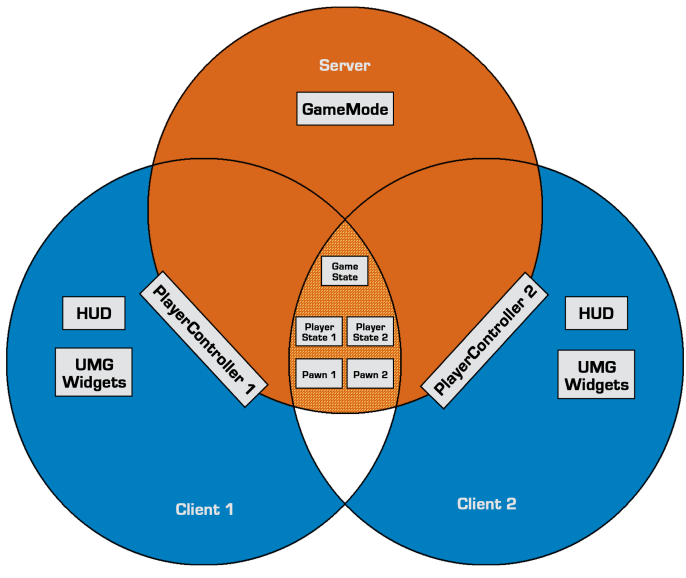
\includegraphics[width=10cm]{./images/ActorsInClientServer.png}
  \caption{Distribución de objetos en un enfoque Cliente-Servidor con \ac{UE4}}
  \label{Objects}
\end{figure}

Para que se pase información entre los clientes y el servidor, es necesaria la \textbf{replicación}. Replicar consiste en el envío de información y datos entre los clientes y el servidor. En \ac{UE4} se puede conseguir la replicación modificando características que afectan a los actores. Para que un actor se replique (aparezca en todos los clientes conectados al servidor) y su movimiento sea igualmente replicado, habrá que añadir las siguientes líneas de código (Listado \ref{LstReplication}) en el constructor del actor:

\begin{lstlisting}[language=c++,caption={Replicación de un actor en C++},captionpos=b,label={LstReplication}]
bReplicates = true;
bReplicateMovement = true;
\end{lstlisting}

De igual forma, se pueden replicar propiedades específicas de los actores, que pueden ser interesantes para el juego. Estas propiedades, en el caso de \textit{Alliance} son la salud del personaje y la estamina, entre otras. Para replicar una propiedad, se añaden las líneas de código del listado \ref{LstHeaderRep} en el fichero de cabecera del actor, y las líneas del listado \ref{LstSourceRep} en el fichero \texttt{.cpp} del actor.

\begin{lstlisting}[language=c++,caption={Fichero de cabecera al replicar una propiedad},captionpos=b,label={LstHeaderRep}]
UPROPERTY(Replicated)
float Health;
UPROPERTY(Replicated)
float Stamina;
\end{lstlisting}

\begin{lstlisting}[language=c++,caption={Fichero fuente al replicar una propiedad},captionpos=b,label={LstSourceRep}]
void AMyPlayer::GetLifetimeReplicatedProps(TArray<FLifetimeProperty>& OutLifetimeProps) const {
    Super::GetLifetimeReplicatedProps(OutLifetimeProps);

    DOREPLIFETIME(AMyPlayer, Health);
    DOREPLIFETIME(AMyPlayer, Stamina);
}
\end{lstlisting}

Un distinto tipo de replicación es la llamada \textbf{\textit{RepNotify}}. En este caso, se hace uso de una función que va a ser llamada en \textbf{todas las instancias} cuando se actualice el valor de la variable. Para utilizar esta replicación, se hace uso del código que se muestra en el listado \ref{lstNotify}.

\begin{lstlisting}[language=c++,caption={Replicación de propiedades con RepNotify},captionpos=b,label={lstNotify}]
UPROPERTY(ReplicatedUsing=OnRep_Health)
float Health;

UFUNCTION()
virtual void OnRep_Health();
\end{lstlisting}

En \textit{Alliance} se ha usado constantemente una forma de replicación, denominada \ac{RPC}. En \ac{UE4} existen tres modelos principales de \ac{RPC}:

\begin{itemize}
\item \textbf{Run on Server}. En este modelo, la llamada al procedimiento remoto es ejecutada sólo en la instancia del actor que se encuentra en el servidor. Sólo se ejecutará un procedimiento de este tipo, si se ha llamado desde el cliente que es el \textit{owner}. Si se llama desde otro cliente, el \ac{RPC} no se ejecuta y se obvia. Este punto será clave en nuestro proyecto.
\item \textbf{Run on owning Client}. En este modelo, la llamada al procedimiento se ejecuta en el \textbf{\textit{owner}} del actor.
\item \textbf{NetMulticast}. En este modelo, la llamada al procedimiento se ejecuta en la instancia del actor que se encuentra en el servidor y se replica después en todas las instancias de los distintos clientes. Para conseguir este comportamiento, la invocación \ac{RPC} se debe realizar desde el servidor, ya que si se realiza desde un cliente, actúa como un procedimiento local, no teniendo en cuenta a los demás clientes. Este punto también será clave en nuestro proyecto. Se puede ver un esquema de este tipo de \ac{RPC} en la Figura \ref{Multicast}.

\begin{figure}[H]
  \centering
  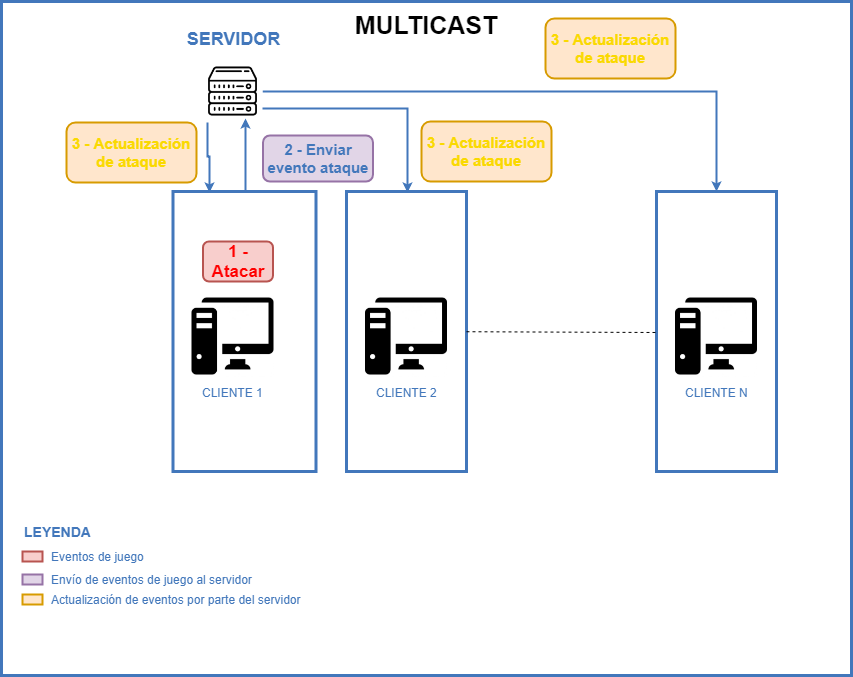
\includegraphics[width=13cm]{./images/Multicast.png}
  \caption{Esquema Multicast en \ac{UE4}}
  \label{Multicast}
\end{figure}
\end{itemize}

\subsubsection{\textit{Ownership}}

La posesión de un actor, es uno de los temas más importantes y que hay que tener más en cuenta a la hora de enfrentarse a un videojuego multijugador. Es importante ya que, como se ha comentado anteriormente, una llamada \ac{RPC} al servidor, se omitirá y no se ejecutará si se llama desde un cliente sobre un actor que no posee. 

Para resolver este problema, se ha seguido el esquema de la Figura \ref{Owning}, ya que la posesión de los actores recae en la instancia del jugador que reside en el servidor. Se comprueba si la llamada a \ac{RPC} del tipo NetMulticast se realiza desde una entidad autoritativa. En \ac{UE4} la autoridad la tiene quien \textit{spawnea} el actor. Si el actor es \textit{spawneado} desde un cliente, la autoridad la tendrá ese cliente. 

En el caso de \textit{Alliance}, los actores a replicar se \textit{spawnean} desde el servidor, y se replican a todos los clientes. Los actores que están colocados en el mundo desde el editor, se encuentran en la categoría <<\textit{placed in world}>>, distinta de la categoría <<\textit{spawned}>>, pero a efectos de replicación, estos actores se tratan como \textit{spawneados} en el servidor.

En el caso de que la llamada se haya realizado por una entidad autoritativa, se puede proceder a realizar la llamada a procedimiento remoto. Si no se ha realizado desde una entidad autoritativa, será necesario que se realice desde el \textit{owner} del actor, que como se ha dicho es la instancia del jugador en el servidor.

\begin{figure}[H]
  \centering
  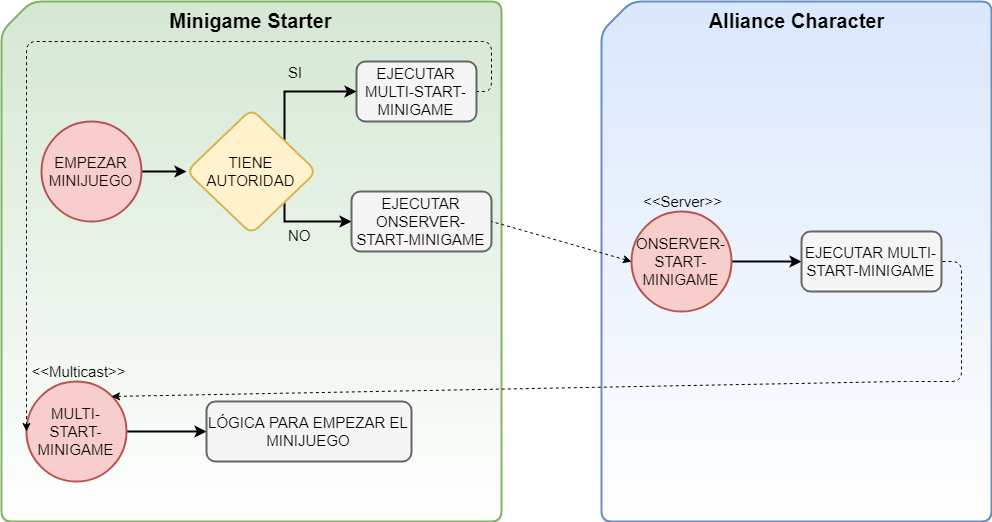
\includegraphics[width=13cm]{./images/Owning.png}
  \caption{\textit{Ownership} en \textit{Alliance}}
  \label{Owning}
\end{figure}
\end{itemize}

\subsubsection{El subsistema online en \ac{UE4}}

El subsistema online (\textit{Online Subsystem}) y sus interfaces, existen para proporcionar una abstracción clara de la funcionalidad online común en todo el conjunto de plataformas disponibles, como pueden ser Steam, Xbox Live, Facebook, etc. Se pretende conseguir principalmente la portabilidad.

Estas plataformas son necesarias, ya que proporcionan un servidor que se encarga de conectar los clientes con la lista de servidores o sesiones de juego disponibles. Además, permiten una visibilidad en internet, que un \textit{host} normalmente no tiene por sí mismo (por ejemplo, por falta de una dirección IP pública fija).

En \textit{Alliance} se ha hecho uso del subsistema online de Steam, por lo que para poder jugar será necesario tener Steam abierto. Al crear una nueva partida, el jugador que lo hace creará una sesión y será el \textit{host} de la partida. Una sesión es una instancia del juego, que se ejecuta en el servidor, con una serie de propiedades como pueden ser el número de jugadores que se aceptan en la partida, si los jugadores se pueden unir a la partida de forma pública o tienen que ser invitados para que puedan entrar, etc. 

Cuando un jugador se une a una partida, el subsistema online busca si existe alguna sesión creada que no se encuentre llena de jugadores. De ser así, pregunta al jugador si quiere unirse y en caso afirmativo, el jugador se une a la sesión que se ha encontrado (se puede ver el flujo de ejecución en el diagrama de la Figura \ref{seqOSS}). En este punto, la sesión estaría llena de jugadores (ya que en \textit{Alliance} se ha establecido un máximo de dos jugadores por sesión), el cliente que se ha unido pasaría a controlar al personaje no controlado por el \textit{host} de la partida, y ambos jugadores podrían comenzar a jugar juntos.

Para el cambio de niveles, se ha optado por destruir la sesión con el nivel actual y crear otra nueva a la que se unirán los dos jugadores. Se ha optado por este método ya que un servidor tiene la capacidad de alojar una sola sesión. Para permitir que se puedan unir varios jugadores a un mismo nivel, al abrir el nivel hay que indicar la opción <<\textit{listen}>>.

\begin{figure}[H]
  \centering
  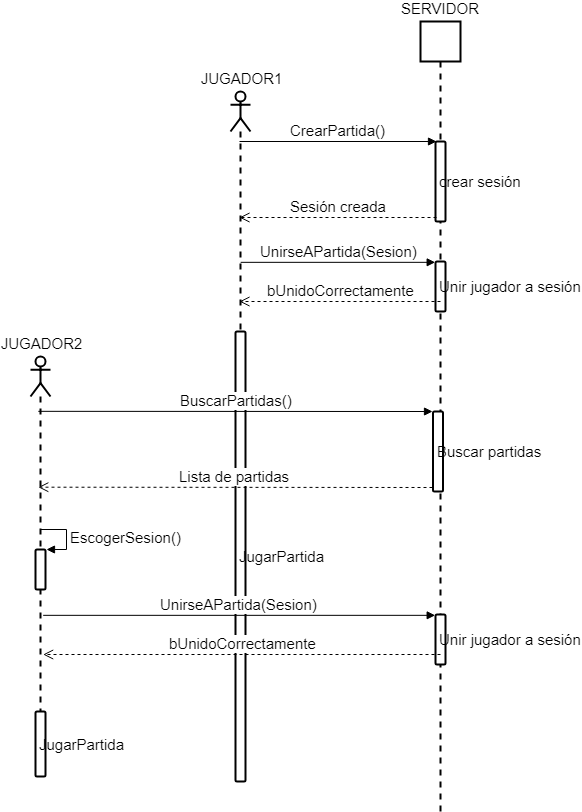
\includegraphics[width=10cm]{./images/Seq_OSS.png}
  \caption{Flujo de conexión de dos jugadores en una partida de \textit{Alliance}}
  \label{seqOSS}
\end{figure}
\end{itemize}


\subsubsection{Elección de personajes en runtime}
En versiones anteriores de \ac{UE4} 4.4 la elección de personajes y, en general, la persistencia de datos entre niveles suponía un gran desafío debido a que no existía la clase \textit{UGameInstance}. 

En estas versiones se optaba por escribir en un fichero de configuración toda la información que debía persistir entre niveles para, una vez cambiado el nivel, volver a importar los valores que se habían escribido en el fichero.
Sin embargo, con la llegada de la versión 4.4 de \ac{UE4} \cite{12} se introdujo la clase \textit{UGameInstance}, esta clase existe tanto en el servidor como en el cliente y puede contener variables replicadas, por lo que es el sustituto perfecto a la anterior solución, mucho más complicada y propensa a errores \cite{13}. \\

Otro desafío a superar era la identificación unívoca de cada cliente a la hora de cambiar de niveles. El método \textitt{PostLogin} de \textit{AGameMode} solamente proporciona el controlador del cliente que se ha unido. \\

Sin embargo, cada jugador tiene un objeto de la clase \textit{APlayerState} asociado, estos objetos están replicados en todos los clientes que estén conectados al servidor y contienen información relevante sobre la red, el jugador y su identificación \cite{13}. Al estar usando el \textit{Online Subsystem Steam} el nombre del jugador asociado es la ID de Steam del jugador, la cual es única para cada jugador. \\

La estructura de datos usada para almacenar esta información ha sido la siguiente:

\begin{lstlisting}[language=c++,caption={Declaración del mapa de jugadores a caracteres},captionpos=b,label={lstAssignedMap}]
TMap<FString, TSubclassOf<AAllianceCharacter>> AssignedCharacters;
\end{lstlisting}

En la cual las claves son los identificadores únicos de Steam y los valores las clases de cada caracter asignado a cada jugador.


A continuación se discutirá la solución propuesta:

El flujo empieza cuando el \textit{AAlliancePlayerController} es spawneado en el mundo y se llama al método \textit{BeginPlay}, dentro de este método se hace una llamada a la \ac{RPC} \textit{OnServerAssignCharacter} el cual tiene la siguiente firma:

\begin{lstlisting}[language=c++,caption={Firma del método OnServerAssignCharacter},captionpos=b,label={lstAssignFirma}]
UFUNCTION(Reliable, Server, WithValidation)
	void OnServerAssignCharacter();
void OnServerAssignCharacter_Implementation();
FORCEINLINE bool OnServerAssignCharacter_Validate() { return true; }
\end{lstlisting} \\

En la firma del método le estamos indicando al \textit{Online Subsystem} de \ac{UE4} que el método se ejecutará en el \textbf{servidor} y será una llamada fiable es decir, que usará un protocolo de transmisión fiable.

Dentro del método \textit{OnServerAssignCharacter} y una vez seguros que todo el código que ejecutemos a partir de ahora se ejecutará en el servidor de la partida:

\begin{lstlisting}[language=c++,caption={Código del método OnServerAssignCharacter},captionpos=b,label={lstAssignCodigo}]
void AAlliancePlayerController::OnServerAssignCharacter_Implementation()
{
	AGameModeBase* GMode = GetWorld()->GetAuthGameMode();
	AAllianceGameMode* Gamemode = Cast<AAllianceGameMode>(GMode);

	if (Gamemode)
		Gamemode->RespawnPlayer(this);
}
\end{lstlisting} \\

Una vez que estamos ejecutando código en el servidor podemos estar seguros de que la llamada a \textit{GetAuthGameMode} no va a fallar \cite{14}. Una vez hemos obtenido y casteado el \textit{GameMode} podemos llamar a la función \textit{RespawnPlayer} pasándole como parámetro el controlador que queremos \textit{spawnear}.

El método \textit{RespawnPlayer} es el encargado de asignar, spawnear y poseer a los caracteres spawneados.

A la hora de programar este método se ha tenido en cuenta de que el juego no sólo debe poder testearse en el modo \textit{standalone}, también en \textit{\ac{PIE}}. Por lo que hay que poner especial cuidado a la hora de prevenir fallos en casos límite como por ejemplo:

\begin{itemize}
	\item Intentar jugar en modo multijugador en el menú principal.
	\item Unirse a una sesión cuando esta ya está empezada.
	\item Asignación doble del mismo personaje debido a errores de timing.
\end{itemize}

Para prevenir fallos en el primer caso límite la solución implementada ha sido rechazar spawnear caracteres si el mapa actual era el menú principal.

\begin{lstlisting}[language=c++,caption={Rechazar el spawneo de caracteres en el menú principal},captionpos=b,label={lstRespawnNoMainMenu}]
FString LevelName = UGameplayStatics::GetCurrentLevelName(GetWorld());

if (LevelName.Contains("Main") || LevelName.Contains("Menu"))
	return;
\end{lstlisting}

Otra opción que se consideró fue retrasar el spawneo del carácter hasta que el servidor empezara una partida pero se rechazó debido a que aumentaba de forma considerable la complejidad de la solución y sería confuso para el jugador.

El siguiente paso es asignar el caracter al jugador, en el caso de que no haya escogido uno anteriormente, los casos en los que podría pasar esto son:

\begin{itemize}
	\item El segundo jugador se está uniendo a la sesión
	\item Acaba de empezar una sesión \ac{PIE}
\end{itemize}

En el primer caso se le asigna al segundo jugador el personaje que está controlado por la IA.
En el segundo caso se le asigna a \textit{Alyssa}, el personaje por defecto.

Después, dependiendo de cuántos caracteres jugables haya en la partida se realizan las siguientes acciones:

\paragraph{Ningún carácter:}

El juego acaba de iniciarse y no hay ningún carácter jugable en la partida. Se deben spawnear ambos caracteres junto con el controlador de IA del personaje correspondiente y poseer a cada carácter.

Para empezar, se buscan todos los actores \textit{APlayerStart} que existan en el nivel, para obtener la posición inicial de spawneo del primer personaje.

Posteriormente se spawnea el personaje que va a ser controlado por el jugador.

\begin{lstlisting}[language=c++,caption={Búsqueda de playerstarts y spawneo de personaje controlado por el jugador},captionpos=b,label={lstRespawnZeroCharsSpawnPlayer}]
TArray<AActor*> FoundPStarts;
UGameplayStatics::GetAllActorsOfClass(GetWorld(), APlayerStart::StaticClass(), FoundPStarts);


APlayerStart* PStart = Cast<APlayerStart>(FoundPStarts[0]);

FActorSpawnParameters SpawnInfo;
SpawnInfo.SpawnCollisionHandlingOverride = ESpawnActorCollisionHandlingMethod::AlwaysSpawn;
AAllianceCharacter* SpawnedCharacter = GetWorld()->SpawnActor<AAllianceCharacter>(AssignedCharacter, PStart->GetActorLocation() , PStart->GetActorRotation(), SpawnInfo);

SecondPlayer->Possess(SpawnedCharacter);
\end{lstlisting} \\

A continuación se procede a spawnear el carácter que será controlado por la IA junto con su controlador, aunque esta vez la posición de spawneo no es el playerstart que mencionamos anteriormente. Sino que se spawnea cerca del primer carácter, esto cubre el otro caso límite nombrado anteriormente, la unión de un jugador cuando la sesión esté empezada. Este comportamiento está implementado en la función \textit{SpawnSecondPLayerNearFirst}.

\begin{lstlisting}[language=c++,caption={Método \textit{SpawnSecondPlayerNearFirst}},captionpos=b,label={lstSpawnSecondPLayerNearFirst}]
AAllianceCharacter * AAllianceGameMode::SpawnSecondPlayerNearFirst(FVector FirstPosition, FRotator FirstRotation, TSubclassOf<class AAllianceCharacter> SecondCharacter)
{
	FVector NewPosition = FirstPosition;
	NewPosition.Y += 250;

	FActorSpawnParameters SpawnInfo;
	SpawnInfo.SpawnCollisionHandlingOverride = ESpawnActorCollisionHandlingMethod::AlwaysSpawn;
	return GetWorld()->SpawnActor<AAllianceCharacter>(SecondCharacter, NewPosition, FirstRotation, SpawnInfo);
}
\end{lstlisting}

Posteriormente se spawnea el controlador de la IA del personaje asociado y se posee el carácter spawneado anteriormente.


\paragraph{Dos caracteres:}

En este caso ambos caracteres están ya en el nivel y otro jugador se está uniendo a la sesión, solo haría falta cambiar el controlador que posee al carácter asociado al nuevo jugador.


\begin{lstlisting}[language=c++,caption={Cambio de controlador del carácter IA},captionpos=b,label={lstRespawnControllerChange}]
AAllianceCharacter* SecondaryCharacter = GetControlledPawnByAI(FoundCharacters);

SecondaryCharacter->GetController()->Destroy();
SecondPlayer->Possess(SecondaryCharacter);
\end{lstlisting} \\

Como se puede ver, en vez de llamar al método \textit{UnPossess} del controlador este se destruye. Esto es debido a un problema encontrado el cual, después de desposeer y volver a poseer el mismo \textit{pawn} por distintos controladores el controlador que deja de poseer sigue enviando órdenes al \textit{pawn} que dejó de poseer. Por lo que, efectivamente, dos controladores están controlando a un mismo \textit{pawn}.

\subsubsection{Problemas que se han encontrado durante la replicación}

Durante el desarrollo de \textit{Alliance} ha habido algunos problemas relacionados con el multijugador y la replicación de los actores. Estos problemas han sido los más costosos de resolver, debido a la dificultad al depurar este tipo de problemas y la falta de información que se encontraba en foros de programación, como son StackOverflow\footnote{https://stackoverflow.com} y el foro de Unreal Engine\footnote{https://forums.unrealengine.com}. En muchos casos, era difícil seguir el flujo de ejecución del programa, por la naturaleza distribuida del videojuego. 

A continuación, se explican los problemas más notables y cómo se han afrontado en el proyecto:

\begin{itemize}
\item Como se ha visto anteriormente, para replicar un actor con apariencia de humano es necesario establecer las propiedades \texttt{bReplicates} y \texttt{bReplicateMovement}. Cuando se lanzaba el juego en multijugador, el jugador que actuaba como cliente (se llamará cliente al jugador que no actúa como \textit{host} y se llamará servidor al jugador que \textit{hostea} la partida) podía moverse pero cuando atacaba o esprintaba, el servidor no veía estos cambios. Para el servidor el jugador se seguía moviendo a velocidad normal y no veía que el cliente atacaba. 

Esto se producía debido a que las animaciones que se dan al esprintar o atacar no estaban siendo replicadas, ya que la llamada a un procedimiento \textit{multicast} desde un cliente, se ejecuta tan sólo localmente en dicho cliente y el comportamiento necesario es que se ejecute en el servidor, y se replique a cada uno de los clientes. Para resolverlo se tomó un enfoque basado en \ac{RPC}, de forma que cuando el cliente ataca, se notifica al servidor que se va a producir este ataque y el servidor se encarga de la replicación de la animación. Si es el servidor el que quiere atacar, se puede ejecutar de forma directa la llamada \ac{RPC} \textit{multicast}. Este enfoque, está basado en la Figura \ref{Owning}.


\item Problemas para lanzar el minijuego desde el cliente, debido a conflictos con el \textbf{ownership}. Cuando se intentaba lanzar el minijuego en el cliente, siguiendo un esquema como el de la Figura \ref{BadApproach}, nos encontrábamos con el problema de que el cliente no podía iniciar el minijuego. Esto es debido a que el enfoque que se siguió es erróneo. La función <<\textit{Server}>> nunca se ejecutaba, ya que era llamada desde un cliente que no es el \textit{owner} del actor, y como se ha explicado anteriormente, este tipo de llamadas se omiten y no se ejecutan.

Para resolverlo, se cambió el enfoque al de la Figura \ref{Owning}, de forma que ahora la función <<\textit{Server}>> sí es ejecutada, porque se llama en el \textit{owner} del actor, que como se ha dicho es la instancia del jugador en el servidor. Desde aquí se llama a la función <<\textit{Multicast}>>, replicando correctamente el funcionamiento.


\begin{figure}[H]
  \centering
  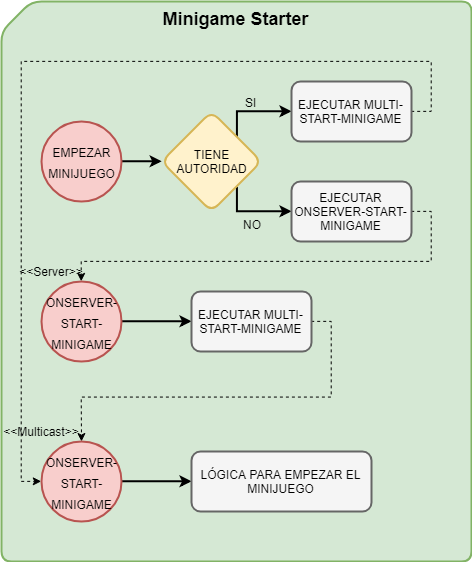
\includegraphics[width=7cm]{./images/BadApproach.png}
  \caption{Enfoque incorrecto al lanzar el minijuego desde el cliente}
  \label{BadApproach}
\end{figure}

\item \textit{Crasheo} del videojuego por un error de violación de segmentos en tiempo de ejecución. Este \textit{crasheo} ocurría al jugar el minijuego cuando un jugador lo había jugado anteriormente.

El error venía causado porque se accedía a una referencia local desde una máquina remota (no tiene sentido compartir una referencia a memoria a un jugador remoto, ya que la memoria de ambos es completamente distinta). Este problema era causado en el evento \texttt{BeginOverlap}. En este evento se toma una referencia al jugador que está haciendo \textit{overlap} (que será quien juega el minijuego), y este evento parecía ejecutarse varias veces, con un comportamiento parecido al de un evento <<\textit{Multicast}>>.

Tras emplear mucho tiempo intentando buscar la solución al problema (para conseguir el comportamiento que se observa en la Tabla \ref{Behaviour}) y no conseguir arreglarlo, se optó por deshabilitar de forma temporal la posibilidad de que el cliente jugase el minijuego, limitando la jugabilidad del mismo al servidor (véase la Figura \ref{Limitation}). Esta no es una opción definitiva (que el cliente pueda jugar el minijuego es una característica muy deseable), por lo que este error se solucionará en actualizaciones futuras. Sin embargo, por el momento no supone un gran problema, ya que aunque el cliente no pueda jugar el minijuego, si que puede observar cómo el servidor lo juega.

\begin{table}[H]
\centering
\begin{tabular}{|c|c|}
\hline
\textbf{Quién juega el minijuego} & \textbf{Comportamiento Deseado}        \\ \hline
Servidor                          & El cliente no puede jugarlo a la vez   \\ \hline
Cliente                           & El servidor no puede jugarlo a la vez  \\ \hline
Cualquiera lo ha jugado           & El minijuego no puede volver a jugarse \\ \hline
\end{tabular}
\caption{Comportamiento deseado del minijuego}
\label{Behaviour}
\end{table}

\begin{figure}[H]
  \centering
  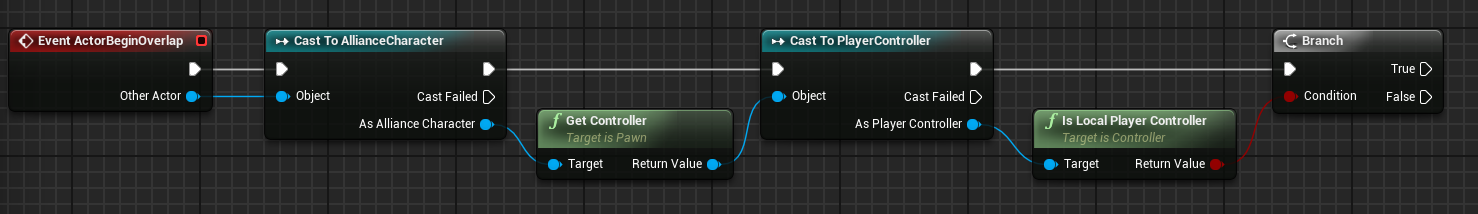
\includegraphics[width=13cm]{./images/LimitacionMinijuego.png}
  \caption{Limitación en la ejecución del minijuego a solo el servidor}
  \label{Limitation}
\end{figure}
\end{itemize}

\subsection{Patrón Observador y Patrón Factoría en la creación de enemigos}

Para \textit{spawnear} los enemigos en el juego, se ha usado un actor a modo de \textit{spawner}, que se encargará de crear los enemigos de cada tipo que se indican por medio de propiedades en el editor. Recibe también como parámetro el número de oleadas de enemigos que aparecerán. Se ha diseñado un esquema basado en el patrón factoría para el \textit{spawn} de los enemigos y basado en el patrón observador para detectar cuando los enemigos de un cierto \textit{spawner} han muerto.

Para crear los enemigos, se usa un \textit{spawner} que comenzará la creación cuando el jugador alcanza una cierta zona del mapa (mediante \textit{overlap} con alguna caja de colisiones invisible). El \textit{spawner} sabe cuántos enemigos de cada tipo tiene que \textit{spawnear} y cuantas oleadas lanzará, pero la creación de los enemigos recae sobre una factoría de enemigos (véase la Figura \ref{Factory}). Esta factoría es la encargada de colocar sobre una determinada posición del mundo a un enemigo de un tipo indicado por el \textit{spawner} y devolverle al mismo el enemigo creado.

 
\begin{figure}[H]
  \centering
  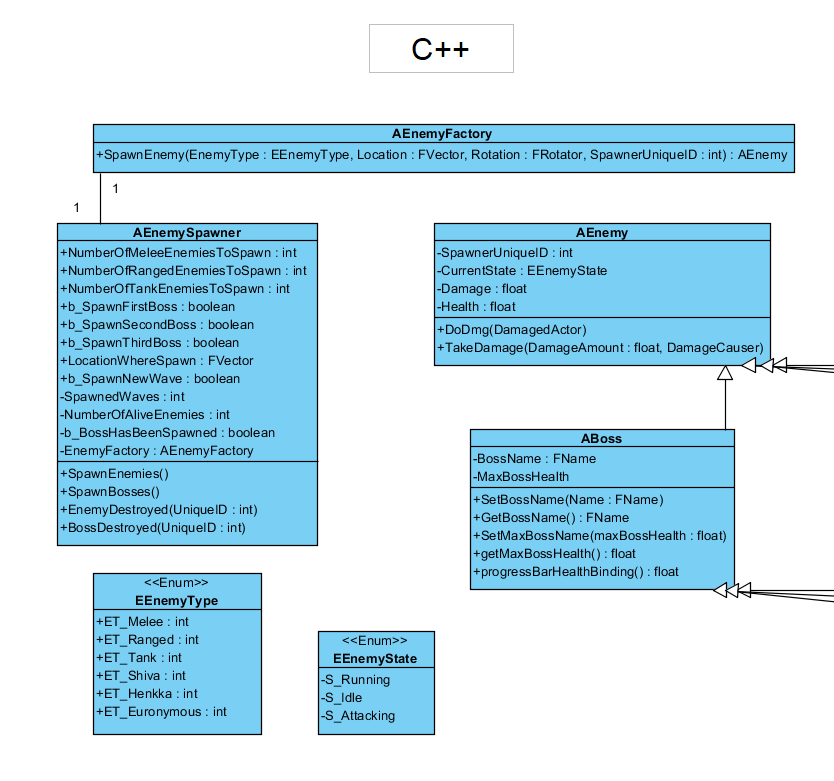
\includegraphics[width=11cm]{./images/FactoryPattern.png}
  \caption{Patrón factoría para la creación de enemigos}
  \label{Factory}
\end{figure}

Para que el \textit{spawner} sepa cuándo un enemigo que ha creado él ha sido eliminado, se usa el patrón observador con delegados (ver Figura \ref{Observer}). En la creación de enemigos, cuando la factoría crea un enemigo, le indica un identificador único que se corresponde con el identificador del \textit{spawner} que lo ha creado. De esta forma, cuando un enemigo muere, notifica mediante el delegado a todos los observadores que ha muerto, usando el identificador que se le ha otorgado. Los \textit{spawner} comprueban si el enemigo que ha muerto ha sido creado por ellos, por medio de este identificador, y de ser así, decrementan su contador de enemigos vivos.

Si este contador llega a cero, significará que todos los enemigos que han creado han sido eliminados. Si quedan mas rondas de enemigos por \textit{spawnear}, procederán a lanzar una nueva ronda de enemigos. Si por el contrario, las rondas de enemigos que el \textit{spawner} tiene que lanzar han sido lanzadas, el \textit{spawner} se destruirá, ya que su labor no es necesaria.

Para acceder a ciertas zonas del mapa que están bloqueadas, es necesario que se hayan eliminado los enemigos de las zonas anteriores. Para llevar a cabo esta comprobación, se mira que los \textit{spawners} de las zonas anteriores hayan sido destruidos. Como se ha dicho, los \textit{spawners} se destruyen una vez que éstos no tienen más enemigos que crear y los que han creado han muerto. Si la comprobación de que los \textit{spawners} de las zonas anteriores están destruidos es cierta, significará que todos los enemigos hasta el momento han muerto.

\begin{figure}[H]
  \centering
  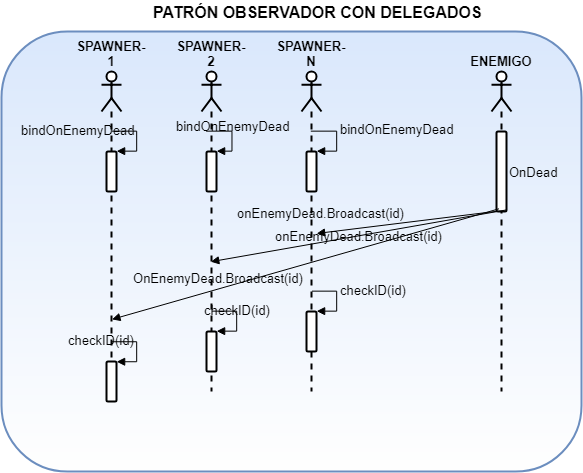
\includegraphics[width=10cm]{./images/Observer.png}
  \caption{Patrón observador en la destrucción de enemigos}
  \label{Observer}
\end{figure}

\subsection{Diálogos en \textit{Alliance}}

Para implementar los diálogos en \textit{Alliance} se ha optado por usar un \textit{plugin}, debido a que el proyecto quedaría mucho más limpio de esta forma y además se ha conseguido un ahorro de tiempo considerable en el desarrollo del proyecto, junto con la facilidad al maquetar los diálogos. El \textit{plugin} se llama \textit{NotYetDialogueSystem} y se puede encontrar de forma gratuita en el \textit{marketplace} de \ac{UE4}\footnote{https://www.unrealengine.com/marketplace/not-yet-dialogue-system}. Se trata de un \textit{plugin} para realizar los diálogos muy potente, basado en una estructura en forma de árbol y orientado a participantes. Esta estructura en forma de árbol se ejecutará de acuerdo a condiciones, que se establecen en los nodos del árbol. Existen varios tipos de nodos, pero los que se han usado para los diálogos de \textit{Alliance} son los nodos de <<discurso>> (o \textit{speech}). A este tipo de nodos se le indica qué texto se mostrará en el diálogo. Entre otras opciones interesantes, cabe destacar el posible uso de archivos de audio en el diálogo, que se reproducirán durante el mismo.

Para establecer los diálogos, es necesario implementar la interfaz que se puede observar en la Figura \ref{Dialog} en la clase del actor participante en el diálogo. Todos los actores que participen en un diálogo deben tener implementada esta interfaz. Una vez que se ha realizado dicha implementación, se pueden usar Blueprints para maquetar estos diálogos, con una estructura en forma de árbol. Aunque se puede hacer el árbol todo lo complejo que se quiera, introduciendo nodos de condición, en \textit{Alliance} se ha optado por seguir una ejecución secuencial, debido a que no era necesario realizar diálogos tan complejos.

Para lanzar los diálogos durante la ejecución del juego, se han usado dos enfoques:

\begin{itemize}
\item Mostrar los diálogos cuando se produce un determinado evento, como puede ser que se haya completado el minijuego correctamente, que se haya eliminado a un jefe final, etc.
\item Mostrar los diálogos cuando se llega a una parte específica del mapa, al hacer \textit{overlap} con alguna caja de colisiones invisible. 
\end{itemize}

\begin{figure}[H]
  \centering
  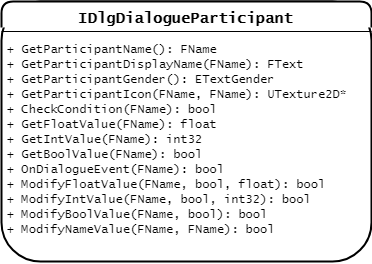
\includegraphics[width=7cm]{./images/IDlgParticipant.png}
  \caption{Interfaz que tienen que implementar los participantes en un diálogo}
  \label{Dialog}
\end{figure}

\subsection{\textit{Breakables} y \textit{Pickups}}

Con el objetivo de incrementar la jugabilidad y teniendo en cuenta que el combate es muy importante en el juego, se ha querido introducir en \textit{Alliance} un mecanismo para conseguir aumentar la vida y la estamina del jugador, mediante la destrucción de ciertos objetos decorativos que se encuentran en el mapa, como son cajas, barriles, carros, etc. 

Estos objetos se han implementado completamente en C++ y otorgan la posibilidad de \textit{spawnear} \textit{pickups} de vida, de estamina o simplemente no \textit{spawnear} nada cuando se rompen. Los objetos decorativos se rompen cuando \textit{Alyssa} ataca con su maza, colisionando con estos objetos o cuando \textit{Morten} dispara sobre los mismos, usando sus armas. Sin embargo, estos objetos no se rompen con los ataques especiales de los personajes, la bola de fuego en el caso de \textit{Alyssa} y la granada en el caso de \textit{Morten}. 

Cabe destacar que ambos actores están completamente replicados, por lo que si el cliente rompe un objeto, el servidor no podrá volver a romperlo ya que observará que ya se encuentra roto (y viceversa). Para conseguir esto, se ha hecho uso de \ac{RPC}, que se ha comentado anteriormente.

La probabilidad de que cuando se rompe un \textit{breakable} se \textit{spawnee} algún objeto de vida o de estamina, se puede poner desde el editor. Se ha hecho así ya que puede ser útil que en un \textit{breakable} concreto se \textit{spawnee} un tipo fijo de \textit{pickup}, por ejemplo el \textit{spawn} de vida en un objeto que se encuentra en un área de combate con jefes enemigos, o el \textit{spawn} de estamina en objetos que se encuentran en los caminos de transición entre distintas arenas. 

Cuando se rompe un \textit{breakable}, al igual que cuando se coge un \textit{pickup} se reproduce un sonido. A estos sonidos, al igual que a los sonidos de los enemigos y personajes, se les ha añadido una atenuación con la distancia, de forma que cuanto más se aleje el personaje de la fuente del sonido, más suaves oirá estos sonidos. Si el personaje está suficientemente lejos, dejará de oír los sonidos gracias a la atenuación. 

\newpage

% Sección 5: Análisis de costes
\pagestyle{insection}
\section{Análisis de costes}
\markboth{Análisis de costes}{}
Como se ha comentado anteriormente, el trabajo desarrollado ha sido una demo jugable de lo que, de continuarse el desarrollo se convertiría en un juego completo.

Debido a esto, se marcó el objetivo de mantener el coste del desarrollo sobre mínimos. Para conseguir cumplir con este objetivo se han llevado a cabo las siguientes acciones:
\begin{itemize}
	\item Usar assets libres o de uso gratis de sitios como el \textit{Unreal Marketplace} o \textit{BlendSwap}.
	\item Usar herramientas colaborativas gratuitas como \textit{GitHub} o \textit{Trello}.
	\item El uso de un motor de juegos gratuito y altamente integrado con el flujo de trabajo que permita no depender de herramientas externas.
\end{itemize}

El desarrollo del proyecto empezó el 27 de mayo teniendo como fecha de finalización el 24 de septiembre, una duración de 121 días de los cuales la dedicación media al proyecto ha sido de 2 h al día. 
Según las últimas encuestas del INE \cite{15} en la que sitúan el sueldo medio de los programadores informáticos en 19,7 \euro/h por lo que el coste de cada programador sería de 4767 \euro.

Teniendo en cuenta todo lo expuesto anteriormente el coste del proyecto ascendería a 14301 \euro \\

\begin{table}[!h]
\centering
\begin{tabular}{cccc}
\hline
\textbf{Concepto} & \textbf{Unidades} & \textbf{Coste Unitario} & \textbf{Coste Total} \\ \hline
Assets            & 0                 &                         & 0 \euro                  \\ \hline
Herramientas      & 0                 &                         & 0 \euro                  \\ \hline
Motor de Juegos   & 0                 &                         & 0 \euro                  \\ \hline
Salario personal  & 3                 & 4767 \euro                    & 14301 \euro               \\ \hline
\textbf{Coste final}       &                   &                         & \textbf{14301 \euro}               \\ \hline
\end{tabular}
\caption{Análisis de costes del proyecto}
\end{table}
\newpage

% Sección 6: Manual de usuario
\pagestyle{insection}
\section{Manual de usuario}
\markboth{Manual de usuario}{}
\subsection{¿Qué hacer si se muestra un error de STEAM al iniciar \textit{Alliance}?}

Si al iniciar \textit{Alliance} nos encontramos con un error como el de la figura \ref{ErrorSteam}, tan sólo tendremos que iniciar sesión en una cuenta de STEAM y reiniciar \textit{Alliance}. El error se debe a que el juego para su funcionamiento online usa el subsistema online de STEAM y sin iniciar sesión en STEAM no se puede hacer uso del mismo.

\begin{figure}[h]
  \centering
  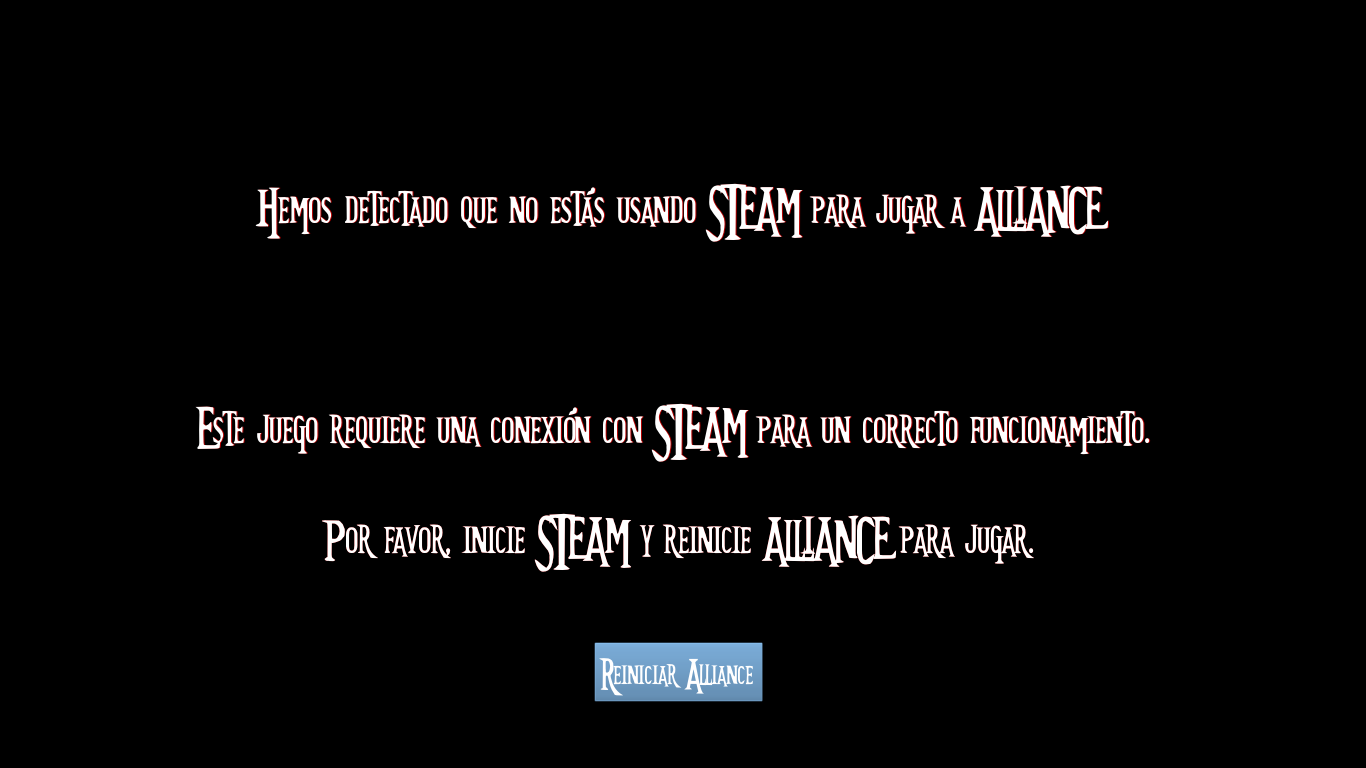
\includegraphics[width=12cm]{./images/ErrorSteam.png}
  \caption{Error de STEAM al iniciar el juego}
  \label{ErrorSteam}
\end{figure}


\subsection{¿Cómo jugar una partida de \textit{Alliance}?}

\begin{itemize}
\item En primer lugar, haz click en el ejecutable de \textit{Alliance}, para iniciar la aplicación.
\item Aparecerá el menú principal del juego, que se puede ver en la figura \ref{MenuPpal}.

\begin{figure}[h]
  \begin{minipage}{0.5\textwidth}
    \centering
    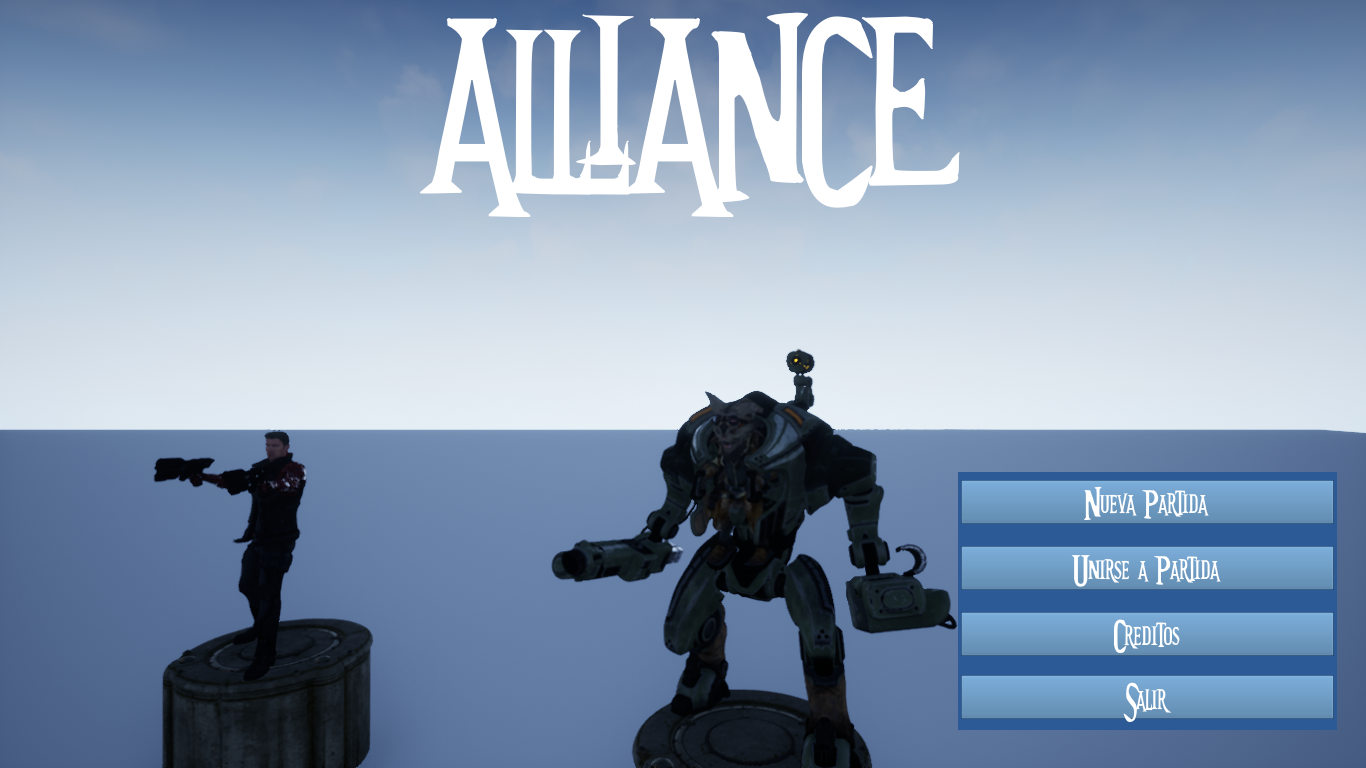
\includegraphics[width=8cm]{./images/MenuPpal.png}
    \caption{Menú principal de \textit{Alliance}}
    \label{MenuPpal}
  \end{minipage}%
  \hspace{1mm}
  \begin{minipage}{0.5\textwidth}
    \centering
    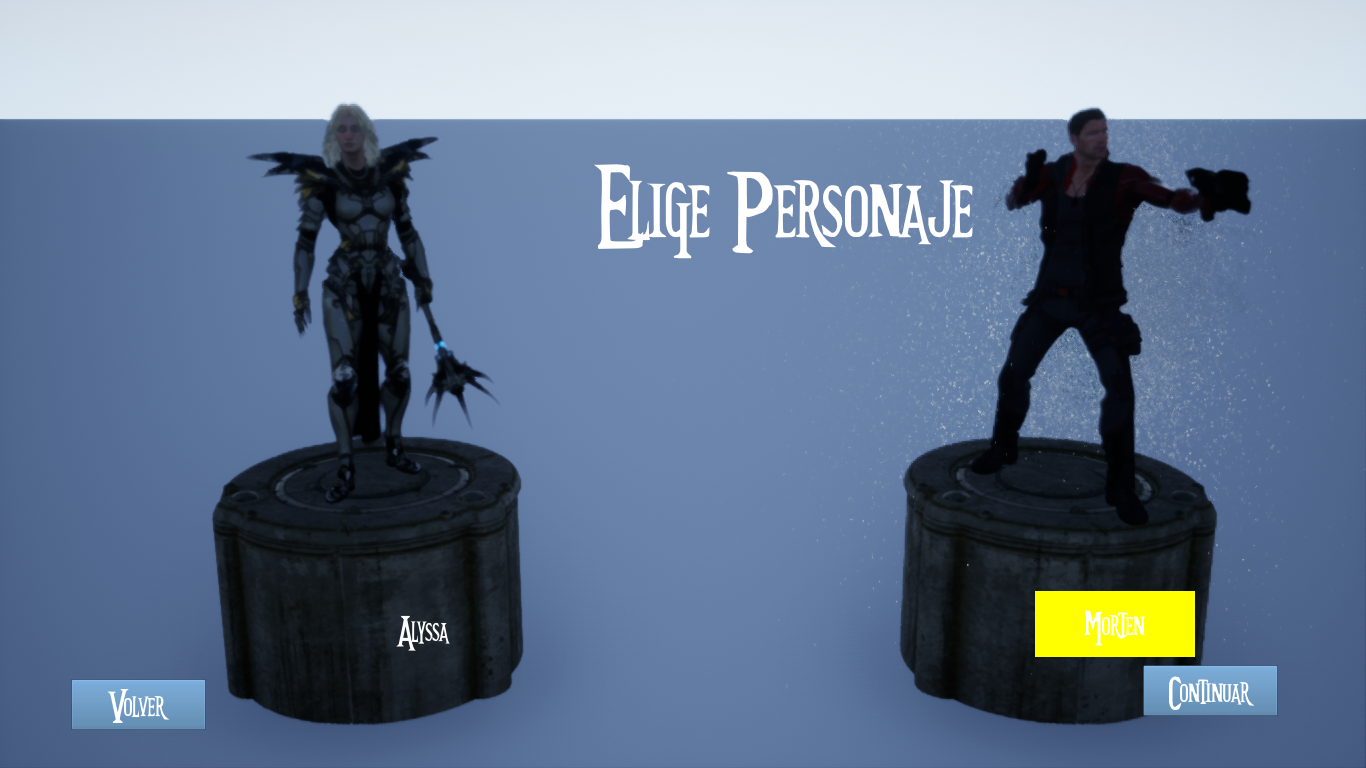
\includegraphics[width=8cm]{./images/EleccPers.png}
    \caption{Elección de personaje}
    \label{EleccPers}
  \end{minipage}
\end{figure}

\item En este menú haremos click en <<Nueva Partida>> para iniciar una nueva partida, la cual vamos a <<\textit{hostear}>>. Esto quiere decir que actuaremos como servidor en el caso de que se una un segundo jugador a nuestra partida. 

\item En la interfaz de la figura \ref{EleccPers}, se puede observar un \textit{zoom} sobre los personajes principales. Elegimos al personaje con el que queramos jugar, haciendo click en el botón con su nombre. Podemos reconocer nuestra selección gracias a las partículas existentes detrás del personaje elegido. 

\item Una vez estemos seguros de la elección de personaje, hacer click en <<Continuar>>. Saldrá una pantalla de carga tras la cual apareceremos en el inicio del primer nivel, y podremos jugarlo.
\end{itemize}


\subsection{¿Cómo unirme a una partida de \textit{Alliance}?}

\begin{itemize}
\item En primer lugar, haz click en el ejecutable de \textit{Alliance}, para iniciar la aplicación.
\item Aparecerá el menú principal del juego, que se puede ver en la figura \ref{MenuPpal}.
\item En este menú haremos click en <<Unirse a Partida>> para unirnos a una partida ya existente.

\begin{figure}[h]
  \begin{minipage}{0.5\textwidth}
    \centering
    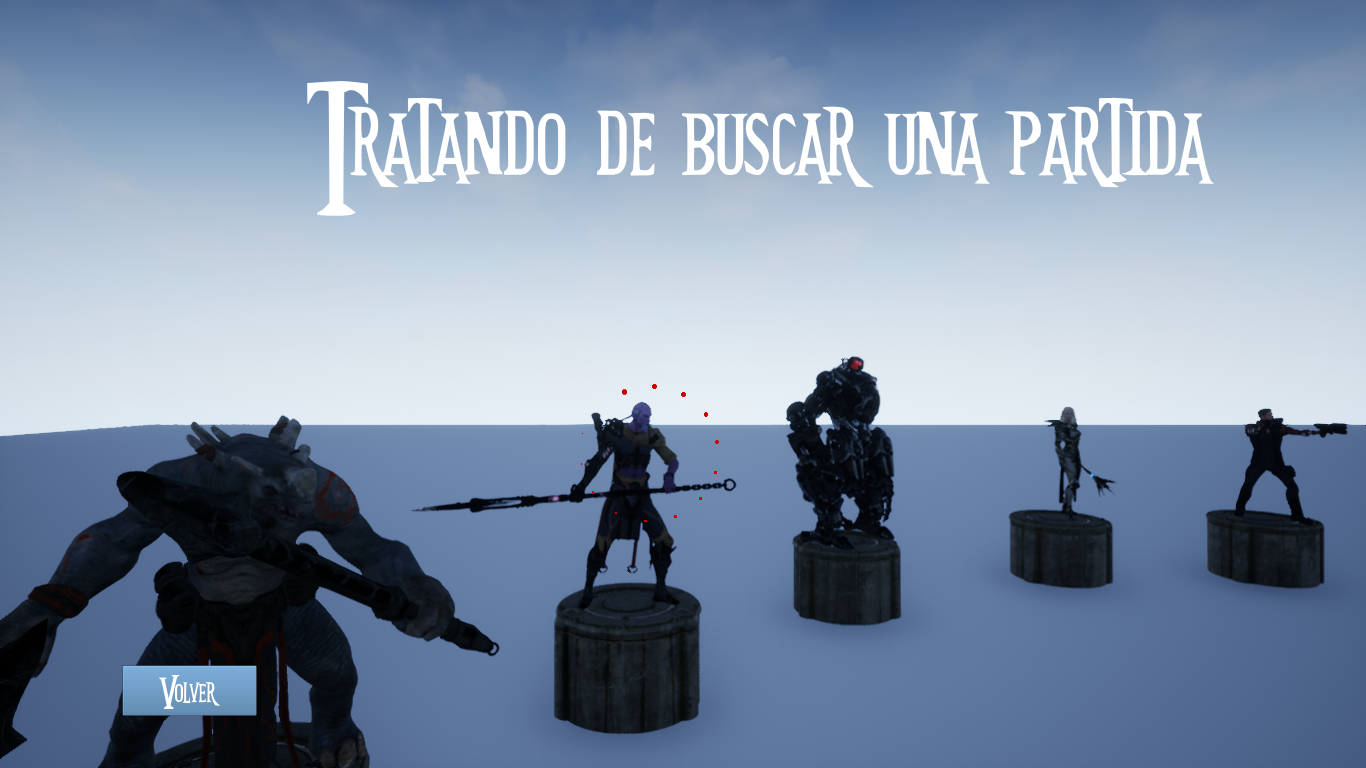
\includegraphics[width=8cm]{./images/BuscandoPartida.png}
    \caption{Buscando partida...}
    \label{BuscandoPartida}
  \end{minipage}%
  \hspace{1mm}
  \begin{minipage}{0.5\textwidth}
    \centering
    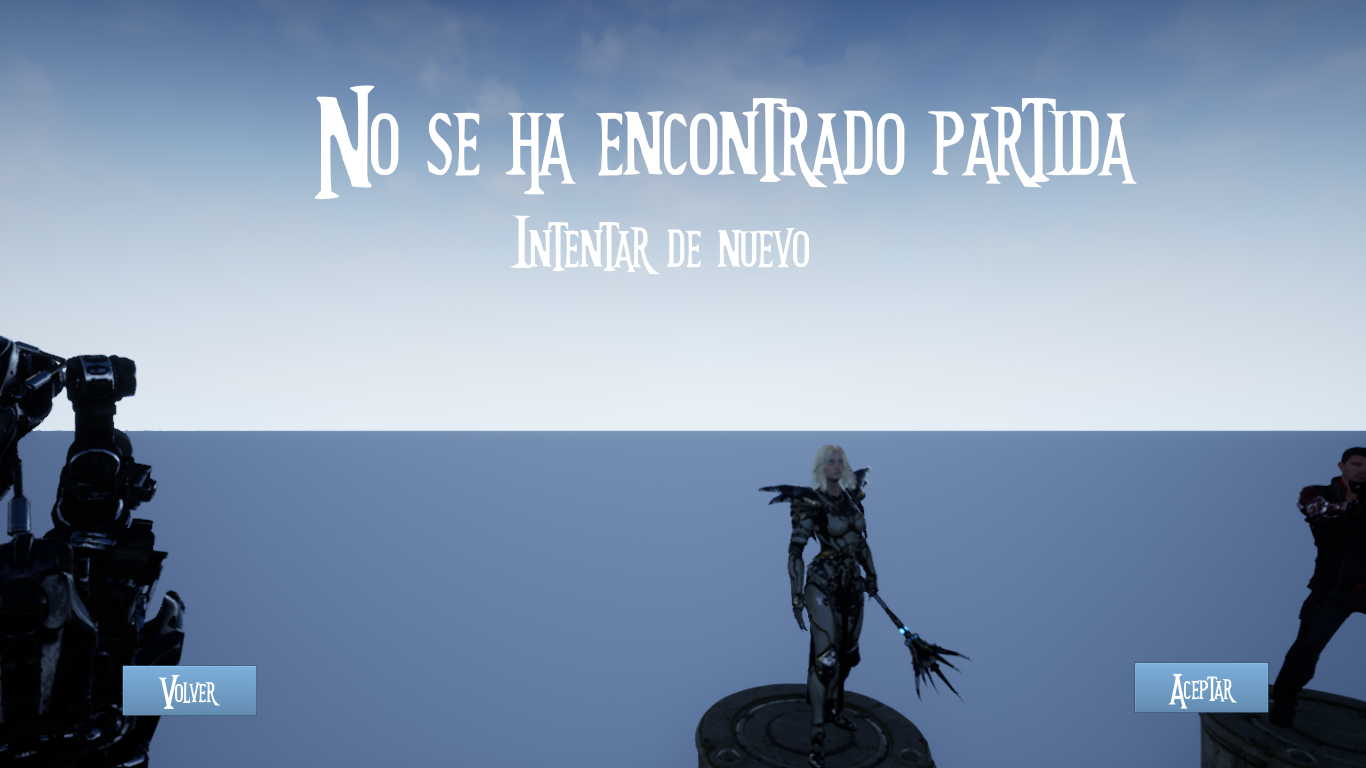
\includegraphics[width=8cm]{./images/PartidaNoEncontrada.png}
    \caption{Error. Partida no encontrada}
    \label{PartidaNoEncontrada}
  \end{minipage}
\end{figure}

\item Inmediatamente \textit{Alliance} comenzará a buscar una partida a la cual puedas unirte, como puede observarse en la figura \ref{BuscandoPartida}. En el caso de que no haya partidas a las cuales puedas unirte, saldrá el mensaje de error que se muestra en la figura \ref{PartidaNoEncontrada}. Puedes realizar una nueva búsqueda haciendo click sobre <<Aceptar>>.

\item Si se encuentra una partida a la cual puedas unirte aparecerá, una pantalla como la de la figura \todo{Insertar figura de éxito al unirse a partida}. Saldrá una cuenta atrás de diez segundos para que aceptes unirte a la partida. Si pasados los diez segundos no te has unido a la partida, deberás proceder a realizar una nueva búsqueda de partidas.

\item Una vez que se ha aceptado unirse a una partida, saldrá una pantalla de carga y tras esta, apareceremos en el nivel en el que se encuentre el jugador que \textit{hostea} la partida, controlando al segundo personaje principal no controlado por el \textit{host} de la partida.
\end{itemize}


\subsection{¿Cómo salir del juego?}

Existen varias maneras de salir del juego, dependiendo de si te encuentras jugando alguno de los niveles de \textit{Alliance}, o si te encuentras navegando por el menú principal (véase Figura \ref{MenuPpal}).

\begin{itemize}
\item \textbf{Si te encuentras navegando por el menú principal.}

Volver hacia las opciones del principio (haciendo click en <<Volver>>), que se muestran en la Figura \ref{MenuPpal}. Una vez en dichas opciones, hacer click en <<Salir>>.

\item \textbf{Si te encuentras jugando alguno de los niveles.}

\begin{itemize}
\item Pausar el juego, presionando la tecla \texttt{P} (o la tecla Escape) y hacer click en <<Salir del juego>>.
\item Dejar que los enemigos nos maten. En la interfaz que aparece (véase Figura \todo{Insertar imagen cuando el jugador pierde}), hacer click en <<Volver al Menú>>. Una vez en el menú principal, escoger la opción <<Salir>>, como se ha indicado anteriormente. 
\end{itemize}
\end{itemize}

\renewcommand\bcStyleTitre[1]{\large\hspace*{1.8in}\textcolor{red!100}{#1}}
\begin{bclogo}[
  couleur=red!15,
  arrondi=0.25,
  logo=\hspace*{1in}\bctakecare,
  barre=none,
  noborder=true]{\hspace*{0.15in} Advertencia.}
\itshape \vspace*{0.15in}
\textit{Alliance} no implementa un sistema de guardado de partidas, por lo que si sales de una partida, no se guardará tu progreso. La próxima vez que inicies \textit{Alliance} deberás empezar una partida nueva, comenzando el juego desde el principio.
\end{bclogo}


\subsection{¿Cómo jugar el minijuego?}

El minijuego que se ha implementado en \textit{Alliance} como mecanismo para abrir ciertas puertas es el clásico <<Klotski>>. Este juego se compone de un tablero, sobre el cual se colocan varias fichas de distintos tamaños y en distintas orientaciones. Existe una ficha, de color rojo (generalmente), que es la que necesitamos mover hacia la salida para ganar. Los únicos movimientos permitidos son horizontales y verticales sobre cada ficha, siempre y cuando haya espacio que lo permita.

En la implementación virtual, existen fichas de colores azules y rojo. La ficha con color rojo es la ficha que hay que llevar al hueco verde para conseguir ganar el minijuego y abrir la puerta. 

Tan sólo se puede mover una ficha si se ha seleccionado. Sabemos si una ficha está seleccionada porque su color cambia a rosa, como se puede ver en la Figura \ref{Minijuego}, y la selección de fichas se realiza pulsando la combinación de teclas \texttt{SHIFT+E} (para seleccionar la siguiente pieza) y \texttt{SHIFT+Q} (para seleccionar la pieza anterior).

Para mover una ficha seleccionada, se usan las teclas \texttt{W} (para mover la ficha hacia arriba), \texttt{S} (para moverla hacia abajo), \texttt{A} (para moverla hacia la izquierda) y \texttt{D} (para moverla hacia la derecha).

\begin{figure}[H]
  \centering
  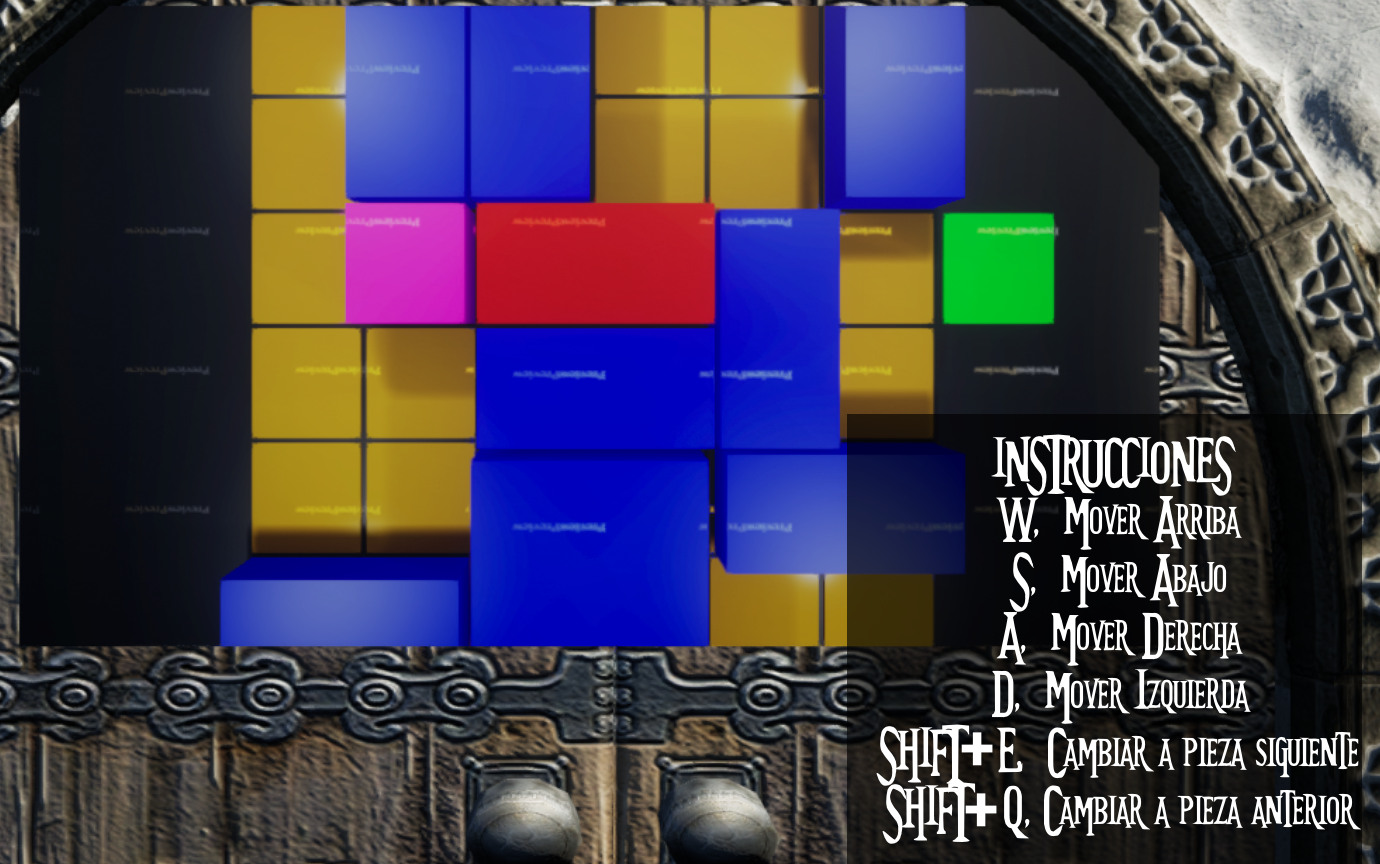
\includegraphics[width=12cm]{./images/Minijuego.png}
  \caption{Ejecución del minijuego durante una partida de \textit{Alliance}}
  \label{Minijuego}
\end{figure}

Durante la ejecución del minijuego, el jugador que lo está jugando no puede moverse ni atacar.


\subsection{¿Cómo incrementar la vida y la estamina?}

La vida y la estamina son los dos rasgos más importantes que posee el jugador. La vida es necesaria para no perder la partida y la estamina es necesaria para poder realizar ataques y para poder correr más rápido. Por esto, se han implementado dos métodos para poder aumentar dichas cualidades.

\begin{itemize}
\item Tanto la vida, como la estamina, se regeneran con el tiempo. Este porcentaje de regeneración es muy bajo, aunque en situaciones de calma en las que no haya combate es muy útil para comenzar los siguientes combates bien regenerado.

\item Existen cajas, barriles y otros destructibles (véase la Figura \todo{Añadir figura de destructibles}). Al romper estos objetos, existe la posibilidad de que aparezcan \textit{pickups} (véase la Figura \todo{Añadir figura de pickups}), que al cogerlos proporcionan vida y estamina.

Coger un \textit{pickup} de vida te aumenta en \todo{Poner cuánto aumenta la salud} puntos tu salud, mientras que coger un \textit{pickup} de estamina aumenta en \todo{poner cuanto aumenta la estamina} puntos tu estamina.
\end{itemize}

\subsection{¿Qué tipos de enemigos existen?}

En \textit{Alliance} hay tres tipos de enemigos principales, además de tres jefes enemigos.

\begin{itemize}
\item Los enemigos principales son:
\begin{itemize}
\item Enemigos a melé (Figura \ref{Mele}). La forma de ataque de estos enemigos es acercarse al jugador más cercano cuando le ven y una vez que están cerca, atacarle. Sus ataques quitan \textbf{x} \unsure{Puntos de vida quita melé} puntos de salud a los personajes controlados por humanos. Tienen una vida total de \textbf{y} \unsure{Puntos de salud tiene melé} puntos de salud.
\item Enemigos a distancia (Figura \ref{Distancia}). Estos enemigos se mantienen a una cierta distancia de los jugadores, desde la que disparan proyectiles en forma de lanza a los mismos. Sus  ataques quitan \textbf{x} \unsure{Puntos de vida quitan enemigos a distancia} puntos de salud a los personajes controlados por humanos. Tienen una vida total de \textbf{y} \unsure{Puntos de salud tienen enemigos a distancia} puntos de salud.
\item Enemigos tanque (Figura \ref{Tanque}). Son enemigos de movimiento y ataque lento, pero muy poderoso. Además pueden recibir mucho daño antes de morir. Su forma de ataque es igual que la de los enemigos a melé, acercándose hacia el jugador más cercano y atacándole. Sus ataques quitan \textbf{x} \unsure{Punts de vida quita tanque} puntos de salud a los personajes controlados por humanos. Tienen una vida total de \textbf{y} \unsure{Puntos de salud tiene tanque} puntos de salud.
\end{itemize}

\begin{figure}[H]
  \begin{minipage}{0.33\textwidth}
    \centering
    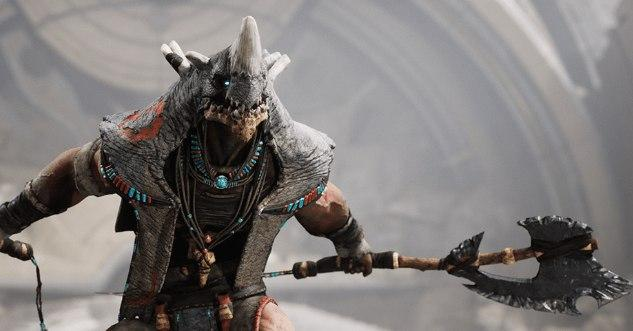
\includegraphics[width=5cm]{./images/guerrero.jpg}
    \caption{Enemigos a melé}
    \label{Mele}
  \end{minipage}%
  \hspace{0.5mm}
  \begin{minipage}{0.33\textwidth}
    \centering
    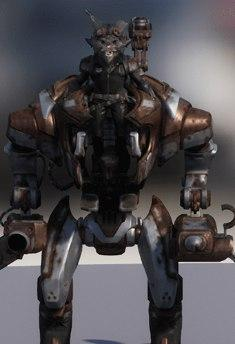
\includegraphics[width=3cm]{./images/distancia.jpg}
    \caption{Enemigos a distancia}
    \label{Distancia}
  \end{minipage}
  \hspace{0.5mm}
  \begin{minipage}{0.33\textwidth}
    \centering
    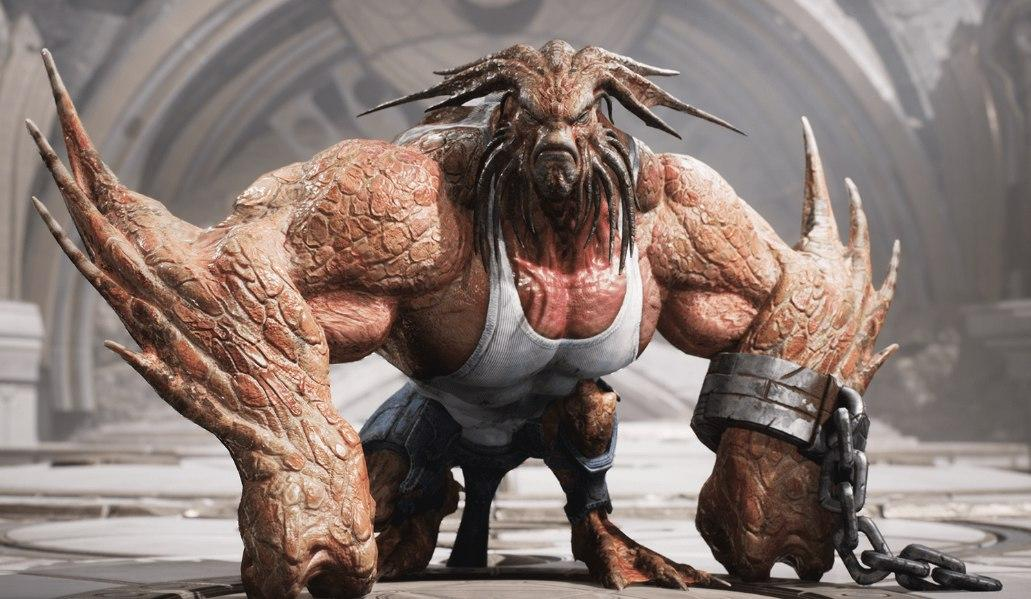
\includegraphics[width=5cm]{./images/tanque.jpg}
    \caption{Enemigos tanque}
    \label{Tanque}
  \end{minipage}
\end{figure}

\item Los jefes enemigos son:
\begin{itemize}
\item \textbf{Henkka} (Figura \ref{Henkka}). Es el jefe de los esclavos de la primera zona. Ataca cuerpo a cuerpo con dos grandes mazas. Sus ataques quitan \textbf{x} \unsure{Puntos que quita Henkka} putos de salud a los personajes controlados por humanos. Tiene una vida total de \textbf{y} \unsure{Puntos que tiene Henkka} puntos de salud.
\item \textbf{Euronymous} (Figura \ref{Euronymous}). Es el jefe de los esclavos de la segunda zona. Ataca cuerpo a cuerpo con una espada, su movimiento es más rápido. Sus ataques quitan \textbf{x} \unsure{Puntos que quita Euronymous} puntos de salud a los personajes controlados por humanos. Tiene una vida total de \textbf{y} \unsure{Puntos que tiene Euronymous} puntos de salud.
\item \textbf{Shiva} (Figura \ref{Shiva}). Es el jefe de los alienígenas enemigos. Sus ataques los lleva a cabo con sus dos grandes puños. Estos ataques quitan \textbf{x} \unsure{Puntos que quita Shiva} puntos de salud a los personajes controlados por humanos. Tiene una vida total de \textbf{y} \unsure{Puntos que tiene Shiva} puntos de salud.
\end{itemize}

\begin{figure}[H]
  \begin{minipage}{0.33\textwidth}
    \centering
    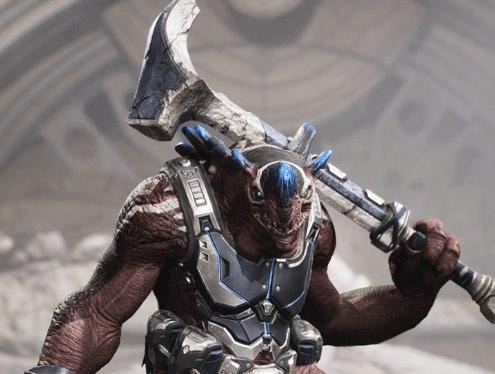
\includegraphics[width=5cm]{./images/henkka.jpg}
    \caption{Boss Henkka}
    \label{Henkka}
  \end{minipage}%
  \hspace{0.5mm}
  \begin{minipage}{0.33\textwidth}
    \centering
    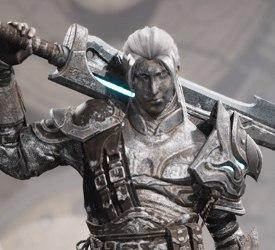
\includegraphics[width=5cm]{./images/euronymous.jpg}
    \caption{Boss Euronymous}
    \label{Euronymous}
  \end{minipage}
  \hspace{0.5mm}
  \begin{minipage}{0.33\textwidth}
    \centering
    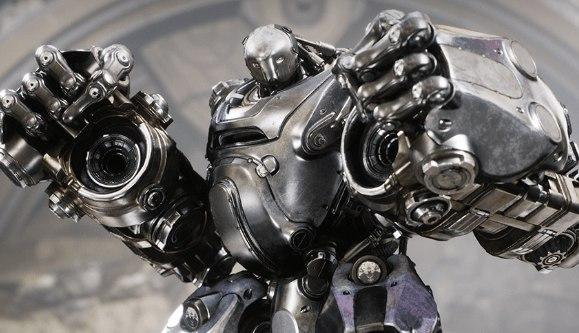
\includegraphics[width=5cm]{./images/shiva.jpg}
    \caption{Boss Shiva}
    \label{Shiva}
  \end{minipage}
\end{figure}

\begin{greenbox}[Sobre el ataque de los enemigos...]
\begin{center}
Todos los ataques de los enemigos quitan una cantidad de puntos de salud a los personajes controlados por humanos. Los personajes controlados por la \ac{IA} no pueden morir, tomen el daño que tomen.
\end{center}
\end{greenbox}
\end{itemize}

\subsection{¿Cómo puedo atacar con \textit{Alyssa}?}

\textit{Alyssa} posee varios ataques, que pueden ejecutarse de las siguientes formas:

\begin{itemize}
\item Ataque básico. En este ataque, \textit{Alyssa} producirá daño golpeando con su maza. Se puede llevar a cabo pulsando el \textbf{botón izquierdo} del ratón. Se pueden encadenar varios de estos ataques en forma de combo, pulsando de forma seguida en repetidas ocasiones este botón.
\item Ataque especial. Si se pulsa el \textbf{botón derecho} del ratón, \textit{Alyssa} lanzará una bola de fuego. Esta bola hace mucho daño a los enemigos, pero también consume mucha estamina.
\item Ataque mientras bloquea. Si mientras se está bloqueando (con la tecla \texttt{F}), se pulsa el \textbf{botón derecho} del ratón, se producirá un daño en área a los enemigos, empujándolos hacia fuera de dicho área. Este ataque es muy útil si nos encontramos rodeados de enemigos.
\item Ataque en carrera. Si se pulsa el \textbf{botón izquierdo} del ratón mientras se está \textit{sprintando} (con la tecla \texttt{SHIFT} pulsada), se producirá un ataque en salto, que es más poderoso que el ataque básico pero a su vez consume mayor estamina.
\end{itemize}

\subsection{¿Cómo puedo atacar con \textit{Morten}?}

\textit{Morten} posee también varios ataques, como son:

\begin{itemize}
\item Ataque básico. En este ataque, \textit{Morten} producirá daño disparando con sus pistolas. Se puede llevar a cabo pulsando el \textbf{botón izquierdo} del ratón. El daño que produce este ataque no es muy alto, pero se ve compensado con la rapidez en la ejecución (lo que permite atacar más veces en el mismo tiempo) y con el poco gasto de estamina.
\item Ataque especial. Si se pulsa el \textbf{botón derecho} del ratón, \textit{Morten} lanzará una granada. Dicha granada explotará pasado un pequeño tiempo, produciendo un gran daño en área a los enemigos que se encuentren dentro del rango de explosión.
\end{itemize}

\begin{greenbox}[Tanto \textit{Alyssa} como \textit{Morten}]
\begin{center}
pueden bloquear ataques pulsando la tecla \texttt{F}, \textit{sprintar} mientras se mueven si se mantiene pulsada la tecla \texttt{SHIFT} y realizar esquivas pulsando el espacio.
\end{center}
\end{greenbox}
\end{itemize}

\subsection{¿Cómo acceder a las partes del mapa bloqueadas?}

En el mapa de \textit{Alliance} existen ciertas partes no accesibles, bloqueadas por un muro invisible como el de la Figura \todo{Figura del muro invisible}. El motivo de este muro es prevenir pasar a algunas zonas sin completar objetivos en las zonas anteriores.

Para poder acceder a las siguientes zonas del mapa, será necesario haber acabado por completo con todos los enemigos de las zonas anteriores. Habremos completado este objetivo si el muro desaparece, permitiendo el paso a la siguiente zona.

\subsection{¿Cómo interactuar con los diálogos?}

Durante el juego aparecerán diálogos, que explicarán la historia del mundo, te guiarán por el camino y te ayudarán con los controles y mecánicas del juego. Estos diálogos tienen la apariencia que se puede observar en la Figura \ref{Dialogo}.

Mientras estás leyendo el texto de los diálogos, el juego estará pausado. Para seguir leyendo el texto, se hará click en la flecha que aparece abajo a la derecha. Cuando no quede más diálogo por leer, este desaparecerá automáticamente y volverás a controlar al personaje principal.

\renewcommand\bcStyleTitre[1]{\large\hspace*{1.8in}\textcolor{red!100}{#1}}
\begin{bclogo}[
  couleur=red!15,
  arrondi=0.25,
  logo=\hspace*{1in}\bctakecare,
  barre=none,
  noborder=true]{\hspace*{0.15in} Advertencia.}
\itshape \vspace*{0.15in}
Cabe destacar que una vez que se ha leído un diálogo, no se puede volver a leer, por lo que ten cuidado al saltarlo y obviar cierta información.
\end{bclogo}

\begin{figure}[H]
  \centering
  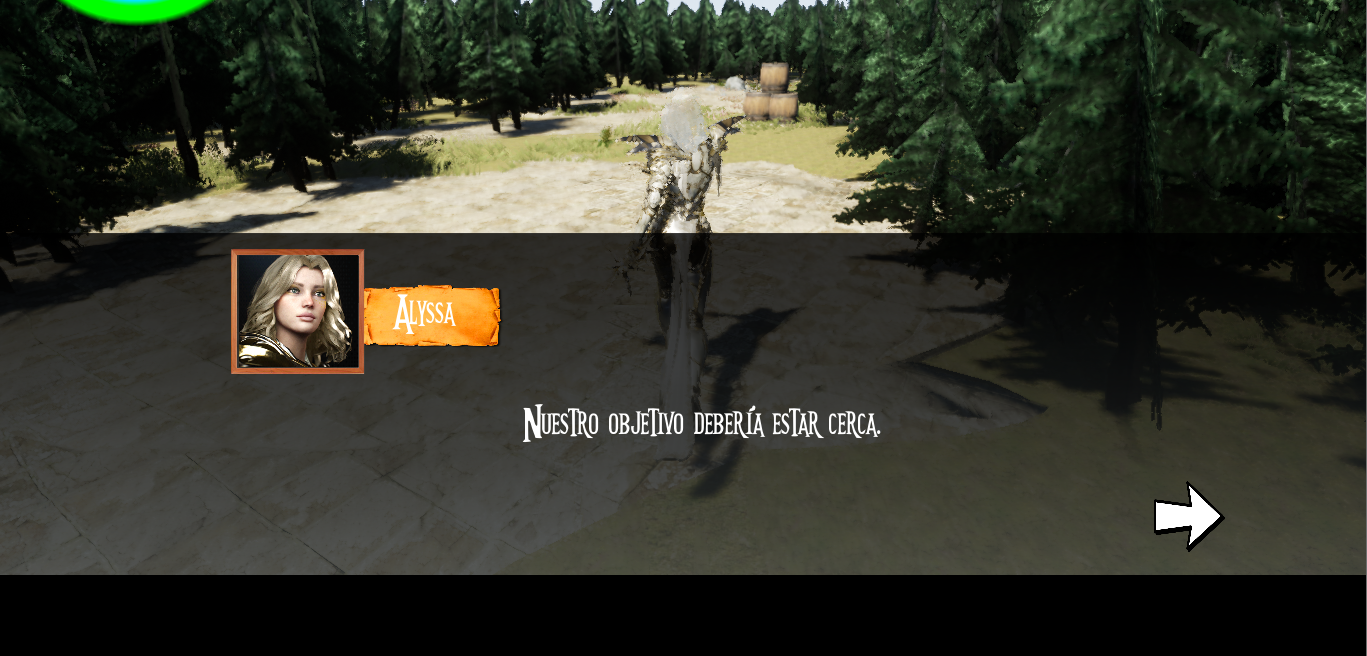
\includegraphics[width=12cm]{./images/Dialogo.png}
  \caption{Interfaz de diálogos de \textit{Alliance}}
  \label{Dialogo}
\end{figure}


\subsection{¿Cómo cambiar el personaje del juego?}

Mientras se está jugando no existe la posibilidad de cambiar el personaje que es controlado por el jugador y continuar con el juego. Existen dos formas de cambiar el personaje, pero ambas necesitan empezar el juego de nuevo:

\begin{itemize}
\item Dejar que los enemigos nos maten. En la pantalla que sale cuando el jugador pierde (se puede ver en la Figura \todo{Insertar imagen cuando el jugador pierde}), hacer click en <<Volver al Menú>>. Una vez en el menú, se puede iniciar una nueva partida escogiendo al personaje que se quiera, entre los dos disponibles.
\item Pausar el juego, presionando la tecla \texttt{P} y hacer click en <<Salir del juego>>. Reiniciar \textit{Alliance} e iniciar una nueva partida, escogiendo al personaje deseado entre los dos personajes disponibles.
\end{itemize}

\renewcommand\bcStyleTitre[1]{\large\hspace*{1.8in}\textcolor{red!100}{#1}}
\begin{bclogo}[
  couleur=red!15,
  arrondi=0.25,
  logo=\hspace*{1in}\bctakecare,
  barre=none,
  noborder=true]{\hspace*{0.15in} Advertencia.}
\itshape \vspace*{0.15in}
\textit{Alliance} no implementa un sistema de guardado de partidas, por lo que si sales de una partida para cambiar tu personaje y empezar una partida nueva, no se guardará tu progreso y tendrás que empezar desde el principio.
\end{bclogo}


\subsection{¿Cómo ver los créditos de \textit{Alliance}?}
\begin{itemize}
\item En primer lugar, haz click en el ejecutable de \textit{Alliance}, para iniciar la aplicación.
\item Aparecerá el menú principal del juego, que se puede ver en la figura \ref{MenuPpal}.
\item En este menú haremos click en <<Creditos>> para visualizar los créditos del videojuego.

\begin{figure}[H]
  \centering
  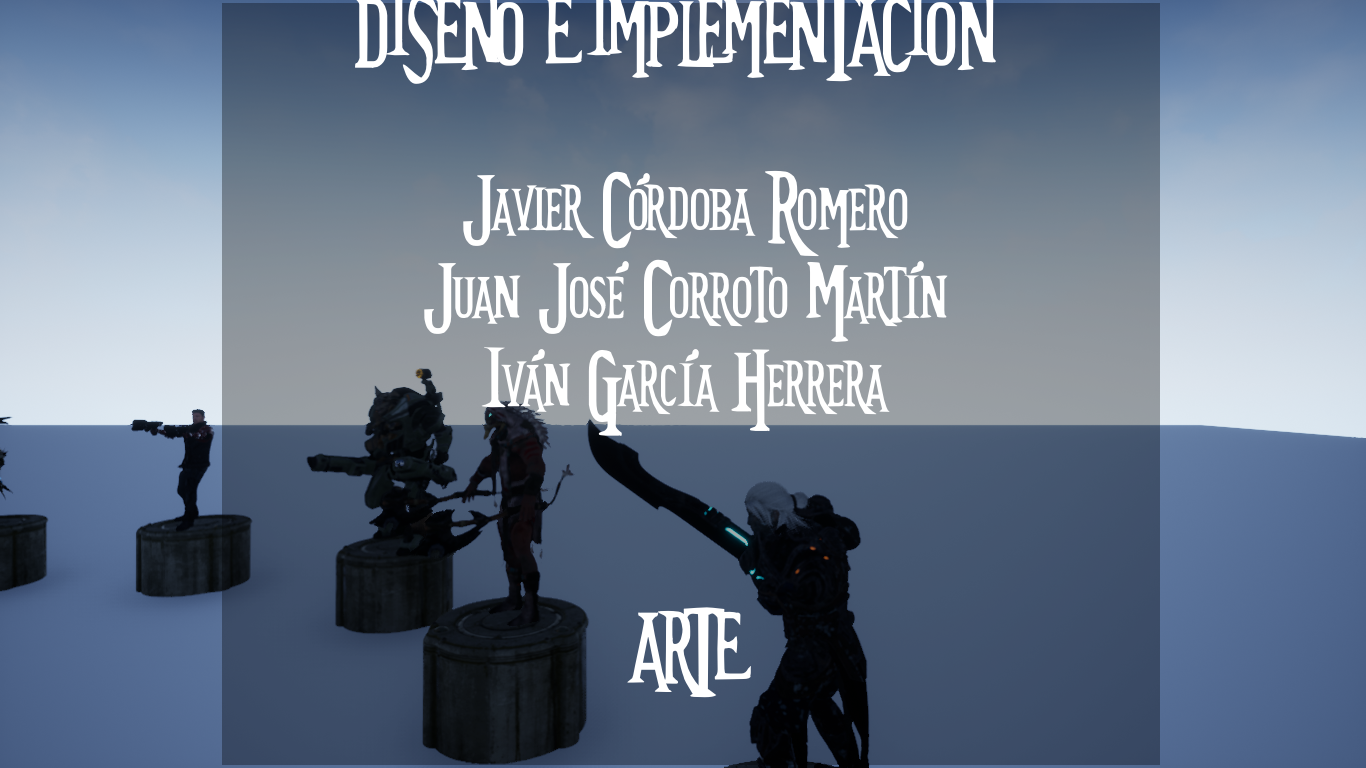
\includegraphics[width=12cm]{./images/Creditos.png}
  \caption{Créditos del juego}
  \label{Creditos}
\end{figure}

\item Se mostrará una interfaz como la de la figura \ref{Creditos}, en la cual se mostrarán los créditos de \textit{Alliance} con una animación de abajo a arriba. Cuando se hallan mostrado todos los créditos, se activará la opción de volver al menú principal del juego.
\end{itemize}

\newpage

% Sección 7: Conclusiones y propuestas de trabajo futuro
\pagestyle{insection}
\section{Conclusiones y propuestas de \\ trabajo futuro}
\markboth{Conclusiones y propuestas de trabajo futuro}{}
El proyecto al final ha resultado ocuparnos más tiempo de lo que habíamos estimado en un principio. Se han finalizado todas las partes importantes que se habían planteado en un principio, pero muchas ideas originales e interesantes que surgían una vez ya estaba empezado el desarrollo (Como la inclusión de un hechizo de curación). Este tipo de cosas no estaban planificadas en un principio, y su inclusión no supone la no realización de los objetivos planteados en la propuesta inicial.
\\

Por otra parte, el género en el que se ha planteado el proyecto se presta más a juegos largos, con más componentes de progresión de los que presentamos en esta solución. Es por eso que el juego se ha planteado más como una forma de \textbf{demostración}. Esto significa que, aunque los elementos principales del juego estén presentes, no se ha pensado en este juego como un producto completo y listo para la venta al público. Aún así, algunos elementos, como es la historia o la eliminación de la progresión, se han adaptado para tratar que parezca un producto un poco más completo, aunque siempre teniendo en cuenta que el juego sería una \textit{demo} de un juego mucho más grande y complejo.
\\

También queremos aprovechar para volver a recalcar lo limitados que nos hemos sentido a la hora de, por ejemplo, trabajar con animaciones preestablecidas. Muchas de las posibilidades en el sistema de combate tuvieron que ser redefinidas cuando empezamos a ver las posibilidades que teníamos a la hora de trabajar con ellas (las animaciones). También nos hemos sentido frustrados frente a la falta de conocimientos que teníamos en ciertos temas como, por ejemplo y sin querer ser redundantes, al trabajar con animaciones. No sabemos si es porque esta parte no es realmente algo que concierne a los programadores(Suponemos que el \textbf{realizar} las animaciones como tal no lo son), pero sí que nos faltaba mucha práctica a la hora de trabajar con ellas, manipularlas y montar todo el sistema de comunicación entre Blueprints que hemos hecho en nuestro proyecto.
\\

Por otra parte, también nos hemos sentido, bien frustrados, bien descontentos, con la inteligencia artificial. En general, nuestra idea de lo que queríamos de inteligencia artificial para los enemigos del juego era más compleja. Al final, quizás por falta de tiempo, o por falta de experiencia o conocimientos, hemos acabado desarrollando una inteligencia artificial más genérica, válida para casi todos los tipos de enemigos con ligeras modificaciones, aunque esa no fuera la idea inicial.
\\

Como propuesta de trabajo futuro, volvemos a reiterar que la idea general del juego es la de una \textbf{demo}. La propuesta de trabajo más inmediata es la de expandir el juego, planteando nuevos mapas y alargando la historia, quizás abandonando la Tierra para perseguir a sus enemigos. Para expandir las mecánicas se puede añadir un sistema de progresión, para desbloquear nuevas habilidades y mejoras (O incluso podemos empezar con algunas de las habilidades especiales de la demo bloqueadas). Otro de los elementos que se deberían mejorar en corto-medio plazo es la inteligencia artificial de los enemigos. No sólo volverla más compleja, si no también evitar ciertos comportamientos poco inteligentes descritos anteriormente. También podrían añadirse nuevos tipos de minijuego, para que no sea siempre el mismo tipo de puzzle.
\\

Algunas posibles mejoras al juego cuando contamos con la ampliación del juego es la inclusión de un modo multijugador para más personas (No sólo dos). Esto supondría que, los aliados que reclutamos en el proyecto que presentamos (Y que recordemos que se trataría como una \textit{demo}), continuarían con nosotros el resto del juego. Además esto supondría también un esfuerzo extra a la hora de diseñar estos personajes, que ahora mismo son tratados como acompañantes que nunca van a ser jugables, y por tanto necesitaríamos hacer más complejo su sistema de combate. También significaría hacer un menú de elección de personaje más complejo, y que aparezca a la hora de unirse a partidas, y diseñar un menú de búsqueda de partidas más adaptado.
\newpage

% Bibliografía/Referencias
\pagestyle{insection}
\markboth{Referencias}{}
\addcontentsline{toc}{section}{\protect\numberline{}Referencias}

\bibliographystyle{plain}
\singlespacing
\bibliography{main}

\end{document}
